\documentclass[11pt]{article}
%\usepackage{acl2015}
%\usepackage{times}
\usepackage{latexsym}
%\bibliographystyle{ieeetr}
\usepackage{amsmath}
\usepackage{multirow}
\usepackage{url}
\usepackage{booktabs}
\usepackage{graphicx}					% to include graphics
\graphicspath{{pics/}}						% folder for graphics
\usepackage{units}
\usepackage{adjustbox}
\usepackage{multicol}
\graphicspath{{pics/}}
\usepackage{tikz}
\usepackage[autostyle=true]{csquotes}
\usepackage{morefloats}



\begin{document}

\section*{Acknowledgments}
A special thanks to my evaluators for their promptness and expertise, and to iCourts, the Danish National Research Foundation's Centre of Excellence for International Courts, for providing me with the data for the European Court of Human Rights.  


\clearpage


\section*{Summary} 
This dissertation presents experiments in which I attempted to automatically extract key phrases from the citation network of the European Court of Human Rights. I employ two different approaches to systematically characterize the citation network of the ECHR by providing scored ngrams, ranked by their propagation in the citation network and by their proportion of times selected through stability selection of randomized logistic regression models of the network. Whereas previous work performing legal network analysis has examined citation patterns, my approach incorporates language use into the study of precedent. The two scoring systems can be used by legal scholars hoping to support their doctrinal analyses with advanced statistical methods of word usage in the citation network of the ECHR. I have also conducted a series of link prediction experiments, showing that textual content is equally, if not more, predictive of citation as metadata and network structure features. \\

A series of validation experiments reveal that my two methods are reliable for capturing citation dynamics within the network. Both experts and I tended to identify trigrams related to Article 10 as relevant when their meme score and stability selection score was higher. The recall and agreement of the annotators was not especially high, however. A validation stage of comparing ngrams with the literature on their respective case law reveals similar patterns. Ngrams matched in the literature had higher scores and ranks than those that did not match. Unmatched ngrams from both the meme score rankings and stability score rankings can be listed on account of their combined ranks and compared to rerankings of different areas of human rights law, in order to gauge which area is understudied. \\


\clearpage
\section{Introduction}
	
	Legal language is known for its use of technical terminology and a level of obscurity that is at times deliberate \cite[p. 3]{tiersma1999legal}. Yet vagueness also serves a purpose in legislation; words meant to regulate an evolving society benefit from allowing multiple interpretations. While the expression ``due process'' and its guarantee of freedom of contract was once used by the US Supreme Court to prohibit minimum wage laws for women, the court later reinterpreted the expression to overturn the opinion \cite{christie1963vagueness}. Judges are therefore tasked with applying an interpretation of the law that hashes out any ambiguity, with some level of consistency, while weighing their words carefully \cite{grundfest2002statutes}. Meanwhile, the professional discourse of the law, courts and legal professionals also requires a precision of communication.  Legal language can also be characterized by pronouncements that need to be clear, internally specific, and at times highly formulaic \cite[p. 3]{tiersma1999legal}. These coexisting traits of legal language --- a vagueness that is addressed explicitly, with definitions aimed at dictating interpretation, and a technical jargon that is used uniquely and routinely --- are an invitation for the use of natural language processing methods and statistical approaches for text analysis. Compared to human dialogue, tweets, or newswire, text that is as formulaic and standardized as legal language can for example, present more reliable results for machine translation \cite{moniapplication}. Similarly, a model such as word2vec, which relies on distributional semantics and the surrounding contexts of words, is well suited for the analysis of legal texts \cite{mikolov2013efficient}. Not only do certain legal systems output a high volume of text data to be used as input, but the contexts used for training are often clarifications and descriptions of the target word itself. \\
	
	
	More generally, advancements in artificial intelligence, information systems and machine learning have found application in the field of legal scholarship and benefit the activities and needs of legal practitioners, as well as the public at large. Since 1987, the biennial conferences of the International Association for Artificial Intelligence and Law and the annual International Conference on Legal Knowledge and Information Systems established the following year have been covering research in the interface of law and technology. The opportunities provided by the coupling of these two fields are abundant and varied. Papers from these conferences or published since 1992 in Artificial Intelligence and Law often involve methods for the modelling of legal argument and reasoning; examining how arguments are put forward and representing the logic involved in solving legal problems \cite{bench2012history}\cite{bench2003model}\cite{ashley2008process}. A vision supported by these endeavours is one in which contracts can be drafted automatically and judgments rendered by AI systems. Many papers otherwise propose new approaches to automate the processing of legal documents, either for classification or summarization, for representing connections between texts or other forms of legal knowledge and informations system management  \cite{vsavelka2015transfer}\cite{buabuchachart2013classification}\cite{galgani2012combining}\cite{bench2012history}\cite{hyman2015process}. Developments in computational approaches applied to these topics are motivated by the ever-growing scale of the law and its complexity. Ontologies of legal concepts, citation networks of judgments, or other natural language processing tools for legal text search have all contributed to making case law and legislation more accessible and understandable, for legal theorists and professionals \cite{getman2014crowdsourcing}\cite{Azzopardi2016}\cite{whalen2016legal}.  \\

The diversity of topics and applications of research in law and AI  is a product of its interdisciplinary nature; computer scientists, legal scholars, linguists and philosophers are all participants in a field that also aims to respond to the needs of lawyers, judges and citizens. While some researchers may use topic modelling techniques to examine the subject matter of court decisions, others may employ text classification to predict the outcome of a case \cite{livermore2015topic}\cite{Ashley2009}.  This contrast has a corollary outlined by political scientists facing the breadth of approaches made possible by computational advances: \begin{quote} \ldots  computer scientists may be interested in finding the needle in the haystack \ldots  but social scientists are more commonly interested in characterizing the haystack \cite[p. 230]{hopkins2010method}.\end{quote}

When legal scholars have made use of developments in computational tools to study the law as a network, through network analysis, collaborations with computer scientists have mainly produced a body of scholarship that relies less on predictions, machine learning, and finding needles, and has prioritized work that characterizes case law, statutes or criminal networks. Legal recommender systems are indeed one focus at the interface of law and AI, and citation networks have proven to be useful for the task of predicting relevant sources of law \cite{winkels2014towards}. Yet networks, and commonly citation networks, have mostly been employed for the insights to be gained from the network's structure and the data it represents. \\

While the links between nodes in a network can represent any kind of relationship (such as followers or contagion) a citation network simply connects judgments to the past opinions they cite.  This kind of relationship can only go in one direction ---constituting a directed rather than an undirected graph --- and there are no cycles looping the network back onto itself; citation networks are ``acyclic'' on account of the relationship represented, namely, a reference to a past judgment \cite{whalen2016legal}. Citation networks support analyses of legal systems in which precedent is central in defining the law \cite{lettieri2016computational}. Countries with a common law system or international courts can produce thousands of judgments, easily amounting to hundreds of thousands of links between nodes in the citation network. Legal network analysis scholarship, as outlined below, has been concerned with making sense of data of this scale, advancing methods that help identify patterns in a hairball shaped haystack.\\

Previous work involving citation networks of judicial opinions has traced the importance of precedent in the US Supreme Court, and how precedent loses value within the court over time \cite{landes1976legal}\cite{black2013citation}. The citation behaviour of judges is theorized in many studies, as citation to precedent is argued to increase for strategic reasons, such as supporting the legitimacy of the court and for persuasion of other judges or involved parties \cite{lupu2010role}\cite{lupu2013strategic}. Network analysis of case law offers tools to systematically represent judicial opinions according to their importance in the jurisprudence. Different centrality metrics have been used to identify which cases are most important based on the the importance of cases that cite them, providing insights on how overruled precedent lose influence or which cases are most likely to be cited in the future \cite{whalen2013modeling}\cite{fowler2007network}. Research has also employed cluster analyses of citation networks, grouping nodes into various communities according to the similarity of information or connectivity of grouped nodes. This approach can demarcate previously undetected areas of the law or identify specific important cases within a legal community that legal scholarship had previously failed to study \cite{mirshahvalad2012significant}\cite{sadl2014empirical}.\\

The use of clustering analysis on citation networks points to one challenge of legal network analysis, namely, how to translate the richness of information offered by a legal citation network into a mapping that is comprehensive and descriptive of the case law in an accessible way. To this end, researchers in information systems and law have also resorted to developments in visual analytics. Recent work has produced an online tool for the analysis of EU case law, combining an interactive citation network toolkit with metadata heatmap and treemap visualization modules to outline the arguments used in the case law \cite{lettieri2016computational}. Similar work has provided a user interface for legal scholars and practitioners to track the path of a single issue in a court's case law, allowing users to navigate both the nodes of the sub network in which the legal issue is captured, as well as the text passages referring to the legal issue \cite{zhang2007semantics}.\\

This representation of jurisprudence in terms of treemaps or paths corresponding to specific issues that can be traced from their point of initial pronouncement to all citing judgments as descendants calls to mind a conceptualization of the law made up of lineages and inheritance.  This analogy has led researchers to characterize the law as genealogy, or in evolutionary terms, as an ever-changing phenomenon subjected to the forces of natural selection \cite{hutchinson2005evolution}\cite{galbraith1988genealogy}.  The proposition that cultural objects such as songs, expressions and habits spread through society, replicating and undergoing mutations precisely as genes do in living organisms was first advanced by biologist Richard Dawkins \cite{dawkins2016selfish}. An evolutionary framing of the law has led legal scholars to pick up on this theory of memetics --- as have social scientists, economists and historians --- to argue that the law carries and transmits legal ``memes'', a parallel to genes \cite{fried1999evolution}. One example is the idiom ``clear and present danger'',  first pronounced by the US Supreme Court to establish a criteria that must be met for the government to limit freedom of speech \cite{strong1969fifty}. This ``meme'' then becomes doctrine, a test to employ for future cases dealing with similar circumstances.  A complete illustration of how the scientific framework of memetics can be supported by the replication of idioms in the citation of precedent (and whether biological phenomena are paralleled in culture as precisely as Dawkins proposes) is outside the scope of this thesis, but has been expanded upon by others \cite{johnson2013memtic}. Nevertheless, the view of citation networks as genealogies characterized by inheritance patterns, from one case to another, of legal language that is unique and formulaic calls for an approach informed by memetics and the study of replication in complex systems other than living organisms.\\

In their own review of legal scholarship employing citation networks, the authors in \cite{sadl2014empirical} lament the overall focus given to studying judicial behaviour and biases. Testing hypotheses about decision-making has been favoured over approaches that analyze the language and legal arguments of the jurisprudence in addition to citation patterns. The authors encourage future work to encompass these three aspects of the data. Notably, on this first aspect, they state: \begin{quote}The analyses of legal language are legion, but the relation of key phrases in jurisprudence to citation patterns and their role in the process of doctrine building are underspecified at best \cite[p. 25]{sadl2014empirical}.\end{quote}

My research takes this account of citation network analysis in legal scholarship as a starting point. As noted above, legal language allows for a high number of key phrases that are constructed and replicated in a standardized manner. My work advances approaches derived from both prediction-focused machine learning research as well as the theory of memetics to exploit the formulaic habits of legal practitioners, while tying citation patterns to a linguistic representation. The combination of natural language processing and network analysis can provide unique insights on the jurisprudence, as the result is a mapping of the case law based on a citation network as well as the language that motivated the reference to precedent.   \\

The data used in this dissertation is a citation network of the European Court of Human Rights (ECHR) and its associated judgement texts. My research attempts to automatically extract key phrases ranked by their relative importance to the case law of the ECHR. I experiment with different methods for scoring relevant ngrams, and various experiments conducted to validate these scores are performed. My scoring of ngrams can provide support to explorations of whether textbooks on the case law are comprehensive or not; a comparison of two textbooks from separate areas of human rights law and their potential omissions outlined by my results suggests one potential application of my method for legal scholarship. \\


Early experimentation with extracting key words from citation patterns of the entire network revealed unigrams that seemed barely interpretable, as seen in table \ref{uni} . This led me to split the citation network into subgraphs specific to the convention Article pertaining to the case (The court considers potential violations of human rights, protected by different  Article in the European Convention on Human Rights). I also focused on retrieving trigram key phrases as a result. The first method involves modelling the citation network and retrieving the text variables that are most predictive of citation.  I begin by conducting various link prediction experiments over the citation network to ensure that the features used for this first method are reliable. A comparison of F-1 scores from logistic regression models trained solely on text content and models including additional features from the network's metadata and structure indicates that accurate predictions can be made with ngrams only. Key phrases are extracted by performing stability selection over several random logistic regression models, trained on the intersection of vocabularies from citing judgments and the precedent they cite. \\

The second method involves combining the frequency of ngrams in the case law with a ratio corresponding to their propagation in the network. Ngrams that appear often in judgments whose cited precedent also contain the ngram, while rarely appearing in judgments that cite precedent with no mention of the ngram, will receive a higher propagation score. This method is meant to extract key phrases that are important to the case law, while also being of particular relevance to that area of the case law. This formula captures the assumed behaviour of memes. Memes are inherited from one judgment to another, as genes are passed on in a lineage. The formula should retrieve the memes that have replicated in the network the most. \\

Both methods, meme scoring and stability selection scoring, share a similar parallel to memetics. There's an inheritance process in citation. My text features for logistic regression models are the shared vocabulary and modelling tells me which is the inherited vocabulary.\\

I conduct several validation experiments to gauge the quality of my ngram scoring through either method. Comparing the scores of ngrams found over those not found in related guidebooks on the case law indicate that both methods have captured some dynamics of citations patterns in the court. Trigrams matched with text in guidebooks are scored higher than trigrams that did not. The evaluation of trigrams retrieved from the Article 10 subgraph, on freedom of expression, by two experts in international law also finds them favouring higher ranked trigrams, for either method. They're agreement and overall recall of trigrams presented to them was low. My own evaluation of a random sample of Article 10 trigrams, based on my interpretation of textbooks on the jurisprudence, confirms my results in a similar fashion. The tirgrams I identify as relevant are ranked higher by both methods over those I ignore. 

\begin{table}[]
\begin{adjustbox}{width=\textwidth}
\begin{tabular}{llll}
\hline
 1.0 2003           & 0.97 particular    & 0.78 arrest       & 0.67 austria      \\
 1.0 77             & 0.96 disputes      & 0.78 company      & 0.67 registry     \\
 1.0 admissible     & 0.96 effective     & 0.78 embodies     & 0.67 vogel        \\
 1.0 adversarial    & 0.95 opponent      & 0.78 slovak       & 0.66 declaring    \\
 1.0 applicability  & 0.92 ordre         & 0.75 appreciation & 0.66 impaired     \\
 1.0 awarded        & 0.91 declared      & 0.75 zlotys       & 0.66 ukraine      \\
 1.0 chamber        & 0.89 obligations   & 0.73 eissen       & 0.65 communicate  \\
 1.0 complexity     & 0.89 turkish       & 0.73 inspire      & 0.65 disorder     \\
 1.0 detention      & 0.88 austrian      & 0.73 liberty      & 0.65 enjoins      \\
 1.0 examined       & 0.88 revision      & 0.73 liras        & 0.65 established  \\
 1.0 laptev         & 0.87 french        & 0.72 maltese      & 0.65 inadmissible \\
 1.0 litigants      & 0.87 quashing      & 0.71 parental     & 0.65 levs         \\
 1.0 mrs            & 0.87 ukrainian     & 0.71 presidium    & 0.64 debts        \\
 1.0 notified       & 0.85 bailiffs      & 0.71 purposes     & 0.64 exhausted    \\
 1.0 question       & 0.84 2007          & 0.71 unilateral   & 0.64 innocent     \\
 1.0 reasonableness & 0.84 series        & 0.69 accused      & 0.64 peaceful     \\
 1.0 redress        & 0.83 organise      & 0.68 innocence    & 0.64 rur          \\
 1.0 reparation     & 0.82 arbitrariness & 0.68 litigation   & 0.63 butkevych    \\
 1.0 speculate      & 0.82 ownership     & 0.68 morals       & 0.63 hedigan      \\
 1.0 states         & 0.82 seeking       & 0.68 appellate    & 0.63 poland       \\
 1.0 tribunal       & 0.81 complained    & 0.68 bulgarian    & 0.63 procedural   \\
 1.0 writing        & 0.81 constituted   & 0.68 expression   & 0.63 wittling     \\
 0.98 editorial     & 0.81 decision      & 0.68 lutkovska    & 0.62 2006         \\
 0.98 fairness      & 0.81 moldova       & 0.68 possessions  & 0.62 principal    \\
 0.97 44704         & 0.79 stake         & 0.67 arguable     & 0.62 quash        \\
\hline
\end{tabular}
\end{adjustbox}
\caption{Unigrams for the entire citation network retrieved by stability selection.}
\label{uni}
\end{table}

\subsection{Contributions}


\begin{itemize}
 \item I perform link prediction experiments over a legal citation network, showing that text content in the legal domain improves the performance of logistic regression models trained without node vocabularies. The F-1 scores of estimators trained only on the intersection of cited and citing judgment vocabularies are mostly higher than for all possible combinations of features related to the network's metadata and structure.
\item I provide a new approach to systematically characterizing a citation network based on the language that is most predictive of citation, by applying a variable selection technique, known as stability selection, to extract ngrams that reflect the case law. This approach can provide a quantitative support to doctrinal analyses of human rights case law, combining citation patterns and the language use associated to them. 
\item A second approach also retrieves and ranks key phrases from the citation network, without performing any modelling of citation patterns. It is the first application of a formula measuring the propagation of a meme in a citation network to be conducted on the case law of the European Court of Human Rights.
\item I provide results from various validation experiments showing the reliability of the two approaches, and suggest a new method for assessing the relative comprehensiveness of textbooks describing the case law. 
\end{itemize}

\subsection{Document Organization}
The rest of this dissertation is organized as follows:
\begin{itemize}
\item Chapter 2 provides a brief outline of the how the European Court of Human Rights and the human rights regime in Europe has developed.
\item Chapter 3 presents past work related to citation networks, my dataset, link prediction and meme detection, outlining the approaches, datasets and results from either article.
\item Chapter 4 goes over my dataset: the ECHR citation network and related guidebooks. The preprocessing steps taken are described along with the character of the data; what a judgment looks like and what the network is composed of.
\item Chapter 5 describes the methods I employ to extract meaningful grams from the citation network: how the meme score is calculated and how logistic regression as well as stability selection are implemented.  The different features used for link prediction are also described.  
\item Chapter 6 outlines the experimental set up for this dissertation. I describe how the link prediction experiments are conducted and how ngram rankings by meme score and stability selection score are retrieved. Different experiments conducted to evaluate these ngrams are described as well.
\item Chapter 7 presents the results of my experiments
\item Chapter 8 analyzes my results. Potential weaknesses in my methods are addressed and ideas for future work are proposed. My results are used for the comparison of jurisprudence textbooks on different areas of the law and the evaluation of their comprehensiveness. 
\item Chapter 9 summarizes the work presented in this dissertation and proposes potential new approaches to be considered for future related work.
\item Chapter 10 provides a overview of the case law for Article 10, as described in a guidebook provided by the court. 
\end{itemize}




\section{Background}
\subsection{History of the European Court of Human Rights}
	Officially inaugurated in 1959, the establishment of the European Court of Human Rights is best understood as both an institution within a nascent legal system and a political project born of the interests of Western Europe and liberal democracy\cite{10.5305/amerjintelaw.105.4.0649}. The court is meant to apply the articles of the European Convention for the Protection of Human Rights and Fundamental Freedoms, entered into force in 1953.  Initially, the court operated in a system that was legally underdeveloped (human rights in Europe) and strongly influenced by national interests. As the court's autonomy grew, a more complete legal system protecting human rights within Europe eclipsed foundational concerns for diplomacy and the threats of fascism, Soviet imperialism and the extensive human rights violations witnessed during World War II \cite{madsen2007cold}.  Today, the combined instruments of the convention and the court, understood as a regime, is considered the most effective in the world \cite{keller2008europe}. The legal dynamics of the regime draws comparisons to a bill of rights (the convention) interpreted and enforced by a nation's constitutional court (Strasbourg)\footnote{One distinction from this comparison can be found in later pronouncements by the court establishing the so-called fourth instance doctrine, namely that the court should not act as final court of appeal, reviewing national courts' potential errors of fact or law \cite{dahlberg2014not}. } \cite{harris2014harris} .  Any of the 800 million individuals from the 47 countries that are party to the convention can appeal to the court when their rights have been violated by their government, hoping to be compensated financially (what the court calls ``just satisfaction'') or to bring about a change in national laws that contravene the convention\cite{boyle2009european}. The court's jurisdiction  has  grown extensively since the convention's ratification in 1953 by a mere 10 states. The fall of the Berlin Wall has seen the membership double, with former Soviet bloc countries become signatories. This history provides for a special development of how Europe came to develop a system to protect human rights, and it is partially outlined below. \\


	A history of strategic Cold War concerns defined the scope of rights considered in the convention\cite{madsen2007cold}\cite{dezalay2006cold}.  A set of human rights covering political and civil life are typically referred to as the first generation of human rights, finding their genesis in political thought of the 17th and 18th century\cite{marks1980emerging}. The majority of the rights protected by the convention fall under this class, such as the right to property, freedom of expression, liberty, life and privacy. The omission of rights belonging to the so called second generation of human rights in the drafting of the convention illustrates some of political priorities of the signatories. In response to accusations levelled at governments of the Soviet bloc, a definition of human rights including social and economic rights such as free healthcare, housing, education and a right to work were promoted by communist regimes and their allies \cite{brander2012compass}. The focus on the first generation of rights reveals the birth of a human rights regime as a product of contemporary political forces:
\begin{quote}
(...)human rights had become a direct battle line in the cultural Cold War of the 1950s and 1960s, seeing the opposing camps of, respectively, the CIA-funded International Commission of Jurists and the Moscow-oriented International Association of Democratic Lawyers fiercely battling over the concept \cite{madsen2007cold}.\\
\end{quote}
	Early pragmatic concerns of legitimacy and precautions taken to not appear as a threat to national interests also advanced certain concepts within the case law\cite{madsen2007cold}. The development of the doctrine of ``margin of appreciation'' is arguably a result of these priorities. A central principle within the jurisprudence of the court, margin of appreciation is a legal device employed to reconcile the impossibility of a universal application of convention articles given specific circumstances a member state may be facing, such as a national emergency or a unique moral landscape \cite{harris2014harris}. The doctrine allows for a certain amount of discretion on behalf of the member states if justified by the particular conditions at the time of the purported violation.\\

	With its legitimacy gradually consolidated, ECHR judges were better positioned to advance jurisprudence in bold directions that allowed for more progressive interpretations of the convention as well as stronger expectations from member states' legal systems \cite{madsen2007cold}. The interpretation of provisions became more forward-looking with a principle establishing that the ``purpose and object'' of the convention be given primacy when the spirit of a case fails to be captured by the exact wording of any provision \cite{harris2014harris}. The convention was subsequently defined as a ``living instrument'' by the court, allowing for a more dynamic interpretation \cite{keller2008europe}. Member states were also expected to provide individuals not only with an abstract recognition of the rights conferred by the convention, but what would be described by the court as a ``practical and effective protection'' of these rights \cite{dzehtsiarou2011european}.\\

\section{Related Work}
\subsection{Empirical Studies of the Webs of International Case Law: A New Research Agenda}
This article maps out a variety of methodologies employed by political scientists and legal scholars to examine the development of case law, especially in international courts, both qualitative and quantitative \cite{sadl2014empirical}. The authors propose an approach that combines citation network analysis, computational linguistics and legal analysis as a new direction for international case law scholarship.\\

	The article sets two branches of case-law scholarship in opposition. One branch represents the political scientist's approach, which operates empirically and quantitatively to focus on the behavior of judges or the outcome of cases, often ignoring the content of the judgment itself. What's in focus is perhaps the judge's professional or ideological background, or the court's motivation for the number of citations used.  The other branch is represented by the legal scholar. The latter can be situated in the ``text book tradition'', updating a record of the important cases pertaining to an area of the law. A legal scholar may also study an important decision in order to clarify the precedent that has been set. The authors point critically to the manner in which many legal scholars are too eager to find congruence between previous practice and legal categories, and what might arise of new case law \cite{sadl2014empirical}.\\

A brief explanation of citation network analysis, its pertinence to the study of the law, and various importance measures is followed by an overview of how citation network analysis has been applied to domestic and international court jurisprudence. A legal theoretical framework is set out in which the interpretation of the law by practitioners and scholars requires a mapping of the case-law that must be comprehensive in order to be correct. The tools outlined in this article provide support for a theoretical framework highlighting the importance of case-law over policy in the application and interpretation of the law \cite{sadl2014empirical}.\\

Despite acknowledging the weaknesses of network analysis (a static picture of the law is posited, and the reason for citation is ignored) the authors advance an approach that builds on previous attempts to combine quantitative methods such as network analysis with qualitative examinations of legal language and argument. More specifically, they perform modularity maximization on a citation network of the Court of Justice of the European Union. This technique, which groups cases into communities according to shared connections, provides the authors with a finding that a central node to one community, ranking high in authority, has gone largely ignored in textbooks. Having made note of the oversight detected through network analysis, an analysis of the case's language is anchored on the presence or absence of a passage involving the word ``effectiveness''. They employ corpus linguistics tools to show that different collocations involving ``effectiveness'' can be juxtaposed with case-law network communities, presenting a systematic study of precedent combining network structure and language \cite{sadl2014empirical}. \\

\subsection{Who Should I Cite? Learning Literature Search Models from Citation Behavior}
The methods in this article are a strong inspiration for my thesis and comes from the field of Natural Language Processing and Information Retrieval. The authors combine information from a citation network, the text content and metadata to produce a retrieval model for the sake of scientific literature search \cite{bethard2010should}. Their features include: 

\begin{itemize} \item A score for the similarity of terms in the query (an article abstract) and the documents (article reference canditates), relying on tf-idf values of the vocabulary.  
 \item The PageRank score of a document, and its citation count, as well as the citation count of its venue, its author, and its author's H-index.
 \item The number of years between the article abstract (the query) and the potential reference.
 \item A similarity score for query terms and document + citing documents terms.
 \item A cosine similarity score for topic distributions vectors of query and document , and a score for query and citing documents
 \item A series of features based on the query author's previous citations, and the names of the author(s) of the query and documents.\\
\end{itemize}
They compare different classifiers for learning the weights of these features, using an iterative approach where sample articles are added to the training data at every iteration, and being compared the training abstract's actual reference list. The classifier iteratively learns what is relevant and what is not and updates the feature weights accordingly, before resampling and retraining. An SVM classifier outperformed a L-BFGS classifier evaluated with mean average precision. Using all features also produced the best results, with citation-count, and topic similarity between abstract and reference candidates(+ reference's citing documents) proving most important \cite{bethard2010should}.\\


\subsection{The Role of Precedent at the European Court of Human Rights: A Network Analysis of Case Citations'}
This article examines the development of precedent at the ECHR and the various political, strategic and legal motivations that factor into the courts decisions \cite{lupu2010role}. \\

Beyond ensuring a consistency in judgments, a court can use precedent in order to legitimize its decision-making and convince parties to follow its judgments and principles. In the case of an international court such as the ECHR, examined by the authors, affected parties are state actors. The court has no mechanism for enforcing its judgments so a domestic court needs to be persuaded by resorting to the legitimacy of existing precedent. A third type of citation practice is said to be influenced by a careful consideration of a nation's interest and how differing morals play against individual rights. This caution is also strategic; the display of sensitivity is necessary to influence the affected government.  These three perspectives (consistency, as well as ``strategic'' and ``relativist'' legitimation) present varying expectations as to why judges cite precedent, how important the cited cases are, and how many cases are cited. Hypotheses as to use of precedent are formulated to test the validity of either perspective \cite{lupu2010role}.\\

The article goes on to describe the data (an ECHR citation network ending at 2006), the distribution of inward and outward citations and their totals over time, how this compares to the US Supreme Court and other figures, i.e. the number of citations and cases, and the distribution of cases across convention articles. \\

The authors arrive at a series of findings that support a perspective in which citation is done to communicate with the involved parties. Hypotheses based on a view in which the purpose of citation is to persuade domestic courts and governments are validated by their research. By examining the characteristics of the cases in the network along with number and importance of cases they cite (hub score), they find that:
\begin{enumerate}
\item violations of convention articles associated to more fundamental issues such as life and torture are backed up by more authoritative cases,
\item these judgments also go on to be more authoritative, i.e. cited heavily 
\item the court relies on precedent more when ruling against a government 
\end{enumerate} 
 
Modularity maximization is performed on the citation network to create communities of citations. They find that the communities are formed around common legal issues rather than being grouped by nation, confirming that 4. the court cites previous cases based on legal substance rather than being concerned with legal culture of a domestic court system and other country-specific characteristics.\\

\subsection{Predicting a Scientific Community's Response to an Article}

This article predicts downloads and citations of articles based on their text content rather than citation network structure as past approaches have \cite{yogatama2011predicting}. They employ supervised learning methods to model the impact of articles, with different modeling approaches for either forecasting or predicting within the same time span as the training data. The prediction task also differs for two datasets; linear regression is used for economics articles whose total number of downloads is modeled whereas a citation network of computational linguistic papers is modeled with logistic regression (either cited or not, three years after publication).\\

The authors go over generalized linear models and penalized regression, especially l2 penalty (ridge regression), which is employed for the non-forecasting predictions task. A novel time-series regularization is applied for the forecasting of citations and downloads. Having split their data by year, the subsequent coefficients for every feature and every year are regularized to control for overfitting as well as variation across years \cite{yogatama2011predicting}.\\

The mean absolute error of their predictions is improved by adding binary indicator vectors of the article texts to metadata features such as author name, conference venue and program name. The time-series regulator offers a small improvement over models trained on all years at once. \\

The advantage of the time-series regularizer is the interpretability of coefficients that captures the importance of ngrams or metadata to the model (and therefore to the scientific community) and its fluctuation over time. The regularization penalty on large variation from year to year results in a smoother timeline, corresponding to research trends, than that of multiple models trained on year-separated datasets (and more informative than the steady coefficient of a model trained on all the data at once). The authors also compare the timelines of a handful of coefficients to timelines illustrating the frequency of these terms in the same literature. Their analysis favors the trends produced by their method, as terms like ``parsing'' and ``grammar'' show more realistic developments \cite{yogatama2011predicting}.\\

\subsection{Inheritance Patterns in Citation Networks Reveal Scientific Memes}

This article employs the understanding of a meme as developed by biologist Richard Dawkins; gene replication and propagation through the gene pool is analogous to a keyword or phrase's distribution in a citation network (as one might also see the sharing of music, ideas or images in culture) \cite{kuhn2014inheritance}. Documents cite each other creating an academic ``bloodline'', in which certain terms may be ``inherited''. A meme refers to terms that are inherited in a more consistent manner, much like genes.\\

The ``meme score'' described by the authors and calculated over various scientific article citation networks is an attempt to identify ngrams that are at once important to the literature while also being interesting. Importance is merely how frequent the meme is, and it is considered more interesting if it has a higher ``propagation score'' in the network. A more detailed explanation of this measure is included in the methodology section below \cite{kuhn2014inheritance}.\\

The authors provide a summary evaluation of this measure through an examination of both frequency ratios and propagation scores of all potential memes across datasets. The similarity in distributions of memes (highly clustered around high propagation and mid to low frequency) is lost when a network is randomized, with nodes assigned random texts. Meme distribution therefore illustrates a process which time and network structure cannot explain on their own. A handful of terms independently hypothesized by the authors as memes, such as ``quantum'' and ``fission'' all share a combined high frequency ratio and propagation score. A more in-depth evaluation follows. \\

The top 50 high-scoring physics memes are mostly deemed relevant to the field by expert annotators, and many appear in Wikipedia physics articles. In a high level of agreement, the two annotators judge the 150 memes with the highest meme-scores to be relevant at a much higher rate than meme's selected at random \cite{kuhn2014inheritance}.\\

A list of ground-truth memes extracted from Wikipedia article titles and links on physics and science is compared to the list of the 5178 highest scoring memes, as well as lists produced with alternatives to the meme score. The alternative metrics are applied in order to examine whether alignment between Wikipedia ``memes'' and results of their meme formula can be reproduced with measures based on different criteria. Scores based on frequency alone, frequency changes over time, and frequency difference across journals exhibit much lower agreement with Wikipedia ground-truth memes. Wikipedia memes also tend to have very high meme score. The authors end with a call for meme identification using more advanced language processing methods, in order to track the inheritance of memes beyond ngram matches.\\


\section{Data}
The entirety of the data used for my experiments consist of a corpus of judgments texts from the European Court of Human Rights and a network representing these judgments and the citations between them. These two datasets were generously provided by the iCourts research centre at the University of Copenhagen. Additional datasets employed in my analyses are a corpus of publications covering the case law related to particular articles of the European Convention of Human Rights.\\

The judgment texts total 17110  documents, mostly in HTML format.  A look at how these judgments are distributed across time reveals a much more active court in recent years: 30 percent of the data consists of judgments from after 2010, 41 percent from between 2000 and 2010 while the first 30 years of the court's history produced 164 judgments, representing 0.0096 percent of the corpus.  \\

An important preprocessing step involved the removal of texts corresponding to the court's decisions rather than judgments. The former purely examines the admissibility of the case and will consequently not go at length into the merits of the case. Every judgment text is made of several parts, each varying in degrees of standardized language. The opening of a judgment lays out the respondent, applicant and which judges are sitting for this particular case.  A ``Procedure'' section establishes when the application originated and the article of the convention that may have been violated.  Under the ``Facts'' heading, the circumstances of the case are explained, often including the trajectory of the case along various national courts. Under the same header, the court will sometimes look at relevant law from the respondent state as well as international law beyond the European Convention on Human Rights. A section entitled ``The Law'' examines the purported violation of the applicant's right, (as it is argued by the applicant and the respondent Government) how the article convention applies to case at hand and how the court has dealt with similar cases in the past. If the case is submitted to the court under many article violations, each violation and article is considered in turn. The court also considers the extent and nature of the compensation awarded to the applicant if a violation of a convention has been found.  Any judge(s) disagreeing with majority opinion of the court will lay out their argument in a dissenting opinion, and possibly in a separate opinion, if a judge is dissenting for reasons that differ from other dissenting judges. Judges can also express their view in ``partly concurring and partly dissenting'' opinions. \\

Although it is possible that judgments may cite previous cases due to these dissenting opinions, I have filtered out these sections from the texts when modeling the court's citations. The sections of a judgment that approach legal boilerplate were kept in with the assumption that a proper model would ignore such linguistic patterns on account of their pervasiveness. \\

Having removed from this corpus the dissenting opinions, decisions, documents in other languages or formats other than HTML, the data is converted to plain text and any reference to a case number or case title is also filtered out so as to avoid predictors that simply result from the citing and cited documents having in their shared vocabulary the title or number of the cited case. In some instances, a case number may correspond to multiple documents, if the court revisits the case in order to handle compensation for a violation, which has not been dealt with. For the sake of my experiments, these resubmissions are ignored. When modeling the texts and their citations I am also limiting my data to judgments that appear in both the citation network and the corpus of judgment texts. After these preprocessing steps, the total count of judgments used is  9923 . \\


The citations between judgments are represented by a directed graph, upon which the modeling of citation is performed. This network has been constructed at iCourts by identifying a variety of citation patterns in the texts: a case number or title is referenced, or paragraphs from the cited text might be mentioned, often in the form of ``(see paragraph)''.  The original graph is composed of 17110 nodes and 92232 directed edges,  where source nodes are the citing case and targets the cited. Node attributes consist of various metadata, some of which is used as features for prediction. The language of the judgment (English or French), the type of document (judgment or grand chamber judgment) and a short string identifying the conclusion reached by the court are all ignored in my feature candidates, as are title and originating body. My experiments do make use of the case's date, respondent country and the article(s) under which the application is submitted. \\

The distribution of cases across countries and across articles is far from uniform. A total of 11129 cases (65 percent of the data) fall under article 6, protecting the right to a fair trial. Italy is the respondent country in 12.6 percent of the cases,1828 of which deal with article 6.  Russia and Turkey are also overrepresented (9.2 percent and 17.4 percent respectively). The court has classified cases according to their level of importance (1,2, 3 or 4), corresponding to the case's contribution to the case-law.  The relative frequency of certain respondent countries or purported article violations can be indicative of applications to the court where the circumstances of the case closely resemble those of existing case-law, and consequently provide little opportunity for the development of the case-law. Their estimated importance is thus also used in this project's experiments. \\

I have created article-specific subgraphs for articles that appear at least 700 times, both as a result of the observing this distribution across articles, and in order to return ranked predictors that would hopefully be more specific to the case-law for each article, while taking into consideration the sufficiency of case numbers and graph edges for adequate modeling. The majority of the cases fall under more than one article, and an analysis of the most common article pairings may be of interest, but I have limited my experiments to articles: 10,  2, 5-3, 8-1, 14, 8, P1-1-1, 5, 3, and 13. The number of edges, representing citations, in these subgraphs range from 40587 to 6483.\\

I have collected a corpus of relevant publications that are affiliated to the court without being binding on its judges. One series, Guides on the Convention, is prepared by the Research and Library Division within the Directorate of the Jurisconsult and is made available on the ECHR website. A second series, Human Rights Handbooks, is made available by the Directorate General Human Rights Council of Europe. Both series cover important cases, discuss how the convention article has been interpreted, and provide insights on how the article ought to be implemented. I have collected 13 of these PDF documents, which I have converted to plain text files. The average publication contains 71 pages and 50 000 words. Article-specific publications from the series often contain in the title ``A guide to the implementation of Article 10 of the European Convention on Human Rights '' \cite{macovei2004guide}. \\
 


\section{Methodology}
I use stability selection combined with L1 logistic regression models to identify variables that are highly indicative of citation. Stability selection is essentially a randomization technique involving the application of a selection algorithm, such as logistic regression. Rather than being applied to the whole dataset, stability selection re-estimates the model many times over different random subsets of the data, drawn without replacement, and with scaled penalties over a random subset of the variables' coefficients . After many iterations, the results are aggregated by detecting which variables are selected at a higher frequency over the subsamples \cite{meinshausen2010stability}.\\

Logistic regression is a discriminative model that estimates P($y|x$) where output is a binary variable. The inner product of the feature vector $x$ and weights $w$ is the first step towards estimating P($y|x$). For my experiments, $y$ refers to a connection in the network between the two nodes that compose the features in $x$ (outlined below). \\
\begin{equation}
	\sum_{i=1}^{N} w_ix_i\\
\end{equation}
\\
This maps f to to a real number, between -$\infty$ and $\infty$. Including this inner product in a logistic function allows for the mapping to fall within the range of [0,1], resulting in actual probabilities\\
\begin{equation}
	p(y = 1|x) = \frac{1}{1 +exp( \sum_{i=1}^{N} w_ix_i)}\\
\end{equation}
\\
The estimation of unknown parameters in a logistic regression model is done with conditional maximum likelihood estimation. The method chooses values for the regression coefficients $w$ that maximize the probability of the training data.
\begin{equation}
\max_{w}\sum_{i=1}^{N}\log p(y_i|x_i,w)
\end{equation}
\\
The maximization will overfit the training data; our model will pick up on noise and find non-existent patterns in the citation network's texts, metadata and network structure. Regularization keeps overly large weights from being learned, by adding a penalty to the maximum likelihood estimation equation, penalizing complexity and controlling the variance. The penalty term here is R($w$)\\
\begin{equation}
\hat{w}=\underset{w}{\operatorname{argmax}}  \sum_{i=1}^{N}\log p(y_i|x_i,w) -\alpha R(w)
\end{equation}
\\
The regularization term R(w) in Ridge regression is the l2 norm of the weights. A higher penalty term leads to lower weights, but never allowing any of the coefficients to get to zero. Thus variables selection is not an option with Ridge regression 
\begin{equation}
\hat{w}=\underset{w}{\operatorname{argmax}}  \sum_{i=1}^{N}\log p(y_i|x_i,w) -\alpha \sum_{i=1}^{N}w_i^2
\end{equation}
\\
L1 regularization, or lasso (Least Absolute Shrinkage and Selection Operator) regression involves a penalty term that sums over the absolute values of the coefficients rather than summing over the squares of the coefficients \cite{tibshirani1996regression}. In this case weights can shrink to zero, allowing for variable selection, although optimization is more difficult.\\
\begin{equation}
\hat{w}=\underset{w}{\operatorname{argmax}}  \sum_{i=1}^{N}\log p(y_i|x_i,w) -\alpha \sum_{i=1}^{N}|w|
\end{equation}
\\
L1 provides sparse weight vectors, many of them set to zero. Fewer features will be used those that correlate are competing for selection. Only one feature will be chosen and one will be ignored. This is overcome with stability selection, as the model is re-estimated many times, resulting in a set of stable variables.\\

\subsection{Bag of Common Words}
The estimator upon which stability selection is performed in order to return ranked predictors is limited to training on features whose interpretation can help explain the court's case-law and that can be automatically matched to text content in literature on the court. I'm performing stability selection on feature vectors corresponding to a ``Bag of Common Words'' between two judgment texts, taken from Node $A$ and Node $B$. Rather than vectorizing each judgment text from the article-specific subcorpus, every feature vector used for modeling describes word occurrences (1 for presence, 0 for absence) shared by two documents, where the length of the vector represents the length of the corpus' vocabulary, with stopwords removed. The intersection of the vocabulary of all texts associated to all connected nodes in the article-specific subgraph makes up half of the data, while the second half is an equal number of vocabulary intersections from pairs of judgment texts sampled at random without replacement, whose nodes in the subgraph are not connected. 

% Definition of circles
\def\firstcircle{(0,0) circle (3cm)}
\def\secondcircle{(0:4cm) circle (3cm)}

\colorlet{circle edge}{blue!50}
\colorlet{circle area}{blue!20}

\tikzset{filled/.style={fill=circle area, draw=circle edge, thick},
    outline/.style={draw=circle edge, thick}}

\setlength{\parskip}{5mm}
% Set A and B
\begin{tikzpicture}

    \begin{scope}
        \clip \firstcircle;
        \fill[filled] \secondcircle;
    \end{scope}
    \draw[outline] \firstcircle node (1) {$ngrams \; A$};
    \draw[outline] \secondcircle node (2){$ngrams \; B$};
    \node[anchor=south] at (current bounding box.north) {$A \cap B $};
\end{tikzpicture}



\subsection{Additional Features}
Metrics related to the textual similarity between judgments, node importance of either judgment in the citation network and metadata revealing commonalities between the cited-citing pairs or important attributes of either judgment are included in my first experiment.\\



\subsubsection{Tf-idf}
One such feature involves the textual similarity between citing and cited judgment, based on the cosine similarity of either document's tf-idf weighted vector representation.\\
Tf-idf term weighting is a method for producing vector representations of documents whereby the terms that are important to that document are given a stronger weight at the index corresponding to that term (instead of a 1 for presence and a 0 for absence). $tf$ refers to the frequency of the term in the document, which will be multiplied by the $idf$, the inverse of that term's frequency in the entire corpus. This controls for words whose high frequency in a document should be unsurprising: common words such as determiners or words such as ``court'' and ``applicant'', which should be found in every document in the corpus. The weight should be higher if a term appears frequently in a  document and if it is specific to it \cite{ramos2003using}. The term frequency is simply the count of the term in the document, logarithmically scaled  \\
\begin{equation}
\mbox{tf}_{t,d} = 1 +\log \mbox{tf}_{t,d} 
\end{equation}

The inverse-document frequency gives us an indication of the term's rarity overall in the corpus $N$, where $df_t$ represents the number of documents containing the term $t$.\\
\begin{equation}
\mbox{idf}_{t,d} =\log \frac{N}{\mbox{df}_t}
\end{equation}
\begin{equation}
\mbox{tf-idf}_{t,d} = (1 +\log \mbox{tf}_{t,d}) \cdot \log \frac{N}{\mbox{df}_t}
\end{equation}
A document is represented as a tf-idf vector, with a length corresponding to the total number of tokens in the corpus, and zeroes where a specific token is absent from the document. The calculated tf-idf value is stored at the index for every term present in the document.\\
The similarity between the vectors for a cited and citing pair is measured by calculating the cosine of the angle between either vector. \\
\begin{equation}
sim(A,B) =cos=\dfrac{A \cdot B}{\vert\vert A\vert\vert  \vert\vert B\vert\vert}
\end{equation}

The numerator of this function is the dot product of either vector, and the denominator is the product of the vectors' Euclidean norms. The cosine similarity measure will be 0 if no words between both documents overlap and 1 if two documents are identical.\\

\subsubsection{Network Analytics}
The authority score of the cited judgment is included as a feature as well.  This is returned by running a Hyperlink-Induced Topic Search (HITS) algorithm over the citation network, producing both authority scores and hub scores. A node with a high authority score is cited by more nodes with higher hub scores. A node with a higher hub score cites more cases with high authority scores. The indegree centrality score included is simply a count of the node's incoming edges.\\


\subsubsection{Metadata}
Four more features included in the full feature set make use of metadata associated to the nodes of the citation network. I've included a feature for the number of days in between the cited and citing judgment, assuming that predicting a link between two judgments ought to be informed by whether the judgment have happened too close together in time. Whether or not the respondent country in the case being cited is the same as the citing judgment was included as well, under the assumption that case law pertaining to the same country might be highly relevant to future judgments.\\

While my modeling is performed over article-specific subgraphs and their associated documents, I am including as an additional feature the number of articles under which the judgment falls that both cases have in common. A case about the right to privacy as well as protection from discrimination should be more likely to cite cases that are submitted under the same articles. Finally the court provides a rating for almost every case, from one to four, indicating its importance to the case-law. The court's importance rating for the cited case in a pair of judgments is used as a feature as well.\\

\subsection{Meme Score}
Inspired by \cite{kuhn2014inheritance}, an additional measure of an ngram's importance within the case law is its ``meme score''. In this instance, no modeling of the citation network or text is performed. The score is calculated by multiplying the ngram's frequency in the subcorpus (associated to the case law covering an article of the convention) and a novel metric proposed by the authors called propagation score. It is essentially a ratio of the judgments that cite case law containing the ngram over judgments that do not. The propagation score is represented by:\\
\begin{equation}
P_m =\nicefrac{\frac{j _m\to m}{j_\to m}}{\frac{j_m\to _n}{j_\to n}}
\end{equation}
the numerator is a ratio of judgments $j$ that contain the ngram (or meme $m$) and cite at least one judgment containing the meme (represented by $j_m\to _m$) over all judgments that cite another containing the meme, $j_\to m$. The denominator is meme-containing judgments whose citations do no contain the meme ($j _m \to _n$) over all judgments that do not cite judgments with the meme ($j_\to n$).\\

The authors in \cite{kuhn2014inheritance} have experimented with different levels of controlled noise $\sigma$ to both perform smoothing as well as filtering out high scoring memes due only to their overall frequency. Their experiments show that $\sigma = 3$ provides best results for their data, and for expediency's sake the same controlled noise will be used in my work. The final meme score is calculated by \\
\begin{equation}
Mm = fm \cdot Pm
\end{equation}
A given meme $m$ is derived by multiplying its relative frequency in the subcorpus with its propagation score. The frequency ratio does not total all counts of the ngram but rather the number of judgments containing the ngram over the number of total judgments.\\

\section{Experimental Set Up}

\subsection{Link Prediction}

A series of link prediction experiments were first conducted in order to compare the performance of an estimator trained purely on textual content (the bag-of-common-words vectors) with an estimator trained on different combinations of metadata, network structure metrics and textual similarity features. This is motivated by the focus on bag-of-common-words vectors in later validation experiments and to ensure that modelling a citation network only with these features is on par with if not outperforming metadata and structure features. \\

\def\firstcircle{(0,0) circle (3cm)}
\def\secondcircle{(0:4cm) circle (3cm)}

\colorlet{circle edge}{blue!50}
\colorlet{circle area}{blue!20}

\tikzset{filled/.style={fill=circle area, draw=circle edge, thick},
    outline/.style={draw=circle edge, thick}}

\setlength{\parskip}{5mm}
% Set A and B
\begin{tikzpicture}

    \begin{scope}
        \clip \firstcircle;
        \fill[filled] \secondcircle;
    \end{scope}
    \draw[outline] \firstcircle node (1) {$ngrams \; A$};
    \draw[outline] \secondcircle node (2){$ngrams \; B$};
    \node[anchor=south] at (current bounding box.north) {$A \cap B \; + \; additional \; features$};
    \draw [->] (2.north) to [out=150,in=30] (1.north);
\end{tikzpicture}



The subgraphs corresponding to Articles 2, 3, 5, 8, 8-1, 10 and P1-1 are used for this experiment. The F1 scores returned on models trained on all possible feature combinations are compared. I am using the Logistic Regression module provided by the Scikit-Learn library \cite{scikit-learn}. Test data is taken from either subgraph by identifying all judgments rendered from 2012 and up. This is motivated by the temporal nature of the citation network, and allows for a link prediction experiment that amounts to a forecasting task. The performance of training only on unigram, bigram and trigram bag-of-common-words vectors is compared to training on the additional features described above. I ran L-1 regularized logistic regression on normalized data corresponding the vocabulary intersections on their own, or along with either of the following features and possible combinations thereof: the number of days between the judgments; whether the judgments deal with the same respondent country; the number of common article violations considered; the importance rating given by the court to the judgment; the cosine similarity of the judgments tf-idf vector representations; the authority and in-degree centrality measures of the cited judgment. \\

The F1-score is taken by calculating the harmonic mean of the model's precision and recall.\\
\begin{equation}
Recall = \frac{True \; Positives}{False \; Negatives + True \; Positives}
\end{equation}

\begin{equation}
Precision = \frac{True \; Positives}{False \; Positives+ True \; Positives}
\end{equation}

\begin{equation}
F1= 2 \cdot \frac{Precision \cdot Recall}{Precision + Recall}
\end{equation}

 \subsection{Ngram Ranking}
Stability selection is performed with RandomizedLogisticRegression from Scikit-Learn \cite{scikit-learn} over trigram bag-of-common-words vectors for Articles 2, 5, 5-3, 8, 8-1, 10, 14 and P1-1-1 and unigram vectors for Articles 2, 3, 5, 5-3, 6, 6-1, 8, 8-1, 10, 13, 14, P-1, P1-1-1. The subset of coefficients whose penalty terms are randomly scaled and the subset of data perturbed at every iteration is sampled at a fraction of 0.75. The scaling of the penalty term is done at 0.5.  200 randomized models are employed for stability selection.Articles whose subgraphs were omitted from stability selection experiments were done so either due to their scale making 200 perturbations unfeasible, or on account of their limited presence in the citation network. This method returns a list of ranked ngram features, ordered by the proportion of times they are selected in the random models. The trigrams extracted and ranked through stability selection are also re-ranked according to their meme-score, calculated by their relative frequency and their ``propagation score'' in their Article-specific subgraph.  \\

\subsection{Evaluation}
The ranked lists of ngrams, as predictors or memes, are first compared to literature on the European Court of Human Rights' case-law. For all ngrams returned, I am looking for matches in ECHR guidebooks on the respective Article or area of the law. The average score of matches, their ranking and their frequency are considered for analysis by comparing to ngrams that were not found in the literature. \\

Additional validation of my ngram rankings and their relation to the case-law is performed by two separate annotation experiments. Both involve a comparison of ngram rankings on Article 10, freedom of expression, and annotators' knowledge of the case-law, with differing degrees of expertise. Having singled out one area of the law, my own judgments on a random selection of Article 10 trigrams is conducted simply by identifying trigrams from the subsample that appear relevant to my interpretation of the case-law, informed mainly by the reading of a 60 page guidebook on the interpretation of Article 10 and a  2007 publication summarizing the case-law on freedom of expression \cite{macovei2004guide}\cite{oetheimer2007freedom}. \\

For the second evaluation experiment, I have recruited two Professors of Law from the University of Copenhagen's Faculty of Law. They were provided with a shuffled selection of Article 10 trigrams, sourced from three sets: the top 50 stability selection predictors, the top 50 memes by meme score, and a  random selection of 100 ngrams, from outside the top 50 ranked trigrams of either list. They were given the following instructions:\\


\begin{quote}There are 193 trigrams (three word sequences) I would like you evaluate. I would like you to answer Yes if you feel that the expression might be important to Article 10 -Freedom of expression- case law. Answer No if you do not see any relevance to the case law, or if you feel the expression would be so pervasive in court judgments that it is not interesting enough.\\ 

My process involved removing stop words, such as ``by'', ``to'', ``for'', etc. This will require that you attempt to infer what may have been in between the words of the trigram, if anything. For example, a trigram extracted from P-1 case law is ``delay paying additional''. This is found in the judgments texts as 
``the national authorities delay in paying the additional compensation'' but other formulations are possible.\\
\end{quote}



\section{Results}
\subsection{Link Prediction: Results} 

The following tables show results for my link prediction experiments over various article subgraphs. The first column of every table shows the F-1 score for models trained only on the binary vectors corresponding to the vocabulary intersections of judgment texts from the cited and citing judgments. No result is provided in the first row of this column, as it indicates scores for models trained without the vocabulary. The second column lists the best F-1 score retrieved from different models. The score can be a result of only the intersection vector, only one additional feature, or any combination of all features. The subsequent seven columns list the average F-1 score returned from models trained only on the intersection vector with that additional feature, as a fraction on the top of the cell. The float listed at the bottom of the cell indicates the average contribution that the feature provides to any other feature combination (ex: the difference between the F-1 score returned by training on the unigram vocabulary intersection with the authority measure of the cited judgment, and the the F-1 score of those features and the cited judgment's in degree score). The final column indicates the F-1 score returned on a model trained on all features (including the ngram vector) \\

\begin{table}[]
\label{my-label}
\centering
\begin{adjustbox}{width=\textwidth}

\begin{tabular}{|c|c|c|c|c|c|c|c|c|c|c|}
\hline
         & Voc-only & Max  & \#Days                                                 & =Cntry                                              & =Artcl                                              & Imprt                                          & Cosine                                               & Auth                                           & Indgr                                               & All  \\ \hline
No vocab &            & 0.8  & \begin{tabular}[c]{@{}c@{}}0.8\\ 0.02\end{tabular}     & \begin{tabular}[c]{@{}c@{}}0.75\\ -0.02\end{tabular}  & \begin{tabular}[c]{@{}c@{}}0.75\\ 0.003\end{tabular}  & \begin{tabular}[c]{@{}c@{}}0.44\\ 0.0\end{tabular}  & \begin{tabular}[c]{@{}c@{}}0.61\\ 0.003\end{tabular} & \begin{tabular}[c]{@{}c@{}}0.8\\ 0.01\end{tabular}  & \begin{tabular}[c]{@{}c@{}}0.8\\ 0.03\end{tabular}     & 0.77         \\ \hline
unigram  & 0.89       & 0.9  & \begin{tabular}[c]{@{}c@{}}0.85\\ -0.017\end{tabular}  & \begin{tabular}[c]{@{}c@{}}0.89 \\ 0.008\end{tabular} & \begin{tabular}[c]{@{}c@{}}0.9\\ 0.01\end{tabular}    & \begin{tabular}[c]{@{}c@{}}0.89\\  0.0\end{tabular} & \begin{tabular}[c]{@{}c@{}}0.89 \\ 0.0\end{tabular}  & \begin{tabular}[c]{@{}c@{}}0.89 \\ 0.0\end{tabular} & \begin{tabular}[c]{@{}c@{}}0.87 \\ -0.012\end{tabular} & 0.87         \\ \hline
bigram   & 0.84       & 0.84 & \begin{tabular}[c]{@{}c@{}}0.83 \\ -0.001\end{tabular} & \begin{tabular}[c]{@{}c@{}}0.84 \\ 0.004\end{tabular} & \begin{tabular}[c]{@{}c@{}}0.84 \\ 0.006\end{tabular} & \begin{tabular}[c]{@{}c@{}}0.84 \\ 0.0\end{tabular} & \begin{tabular}[c]{@{}c@{}}0.84 \\ 0.0\end{tabular}  & \begin{tabular}[c]{@{}c@{}}0.84 \\ 0.0\end{tabular} & \begin{tabular}[c]{@{}c@{}}0.82 \\ -0.009\end{tabular} & 0.84         \\ \hline
trigram  & 0.81       & 0.84 & \begin{tabular}[c]{@{}c@{}}0.81 \\ -0.004\end{tabular} & \begin{tabular}[c]{@{}c@{}}0.81\\ 0.001\end{tabular}  & \begin{tabular}[c]{@{}c@{}}0.82 \\ 0.016\end{tabular} & \begin{tabular}[c]{@{}c@{}}0.81\\ 0.0\end{tabular}  & \begin{tabular}[c]{@{}c@{}}0.81 \\ 0.0\end{tabular}  & \begin{tabular}[c]{@{}c@{}}0.81\\ 0.0\end{tabular}  & \begin{tabular}[c]{@{}c@{}}0.81\\ -0.008\end{tabular}  & 0.84         \\ \hline
\end{tabular}
\end{adjustbox}
\caption{F1 Score of Logistic Regression predictions for Article P1-1 subgraph and associated ngram bag-of-common-words vectors, metadata and network structure features. Second float is feature's contribution to other combinations}
\end{table}

\begin{table}[]
\label{my-label}
\centering
\begin{adjustbox}{width=\textwidth}
\begin{tabular}{|c|c|c|c|c|c|c|c|c|c|c|}
\hline
         & Voc-only & Max  & \#Days                                               & =Cntry                                                & =Artcl                                                 & Imprt                                               & Cosine                                                  & Auth                                                    & Indgr                                                 & All  \\ \hline
No vocab &          & 0.84 & \begin{tabular}[c]{@{}c@{}}0.84\\ 0.047\end{tabular} & \begin{tabular}[c]{@{}c@{}}0.79\\ -0.005\end{tabular} & \begin{tabular}[c]{@{}c@{}}0.69\\  -0.002\end{tabular} & \begin{tabular}[c]{@{}c@{}}0.43\\ 0.0\end{tabular}  & \begin{tabular}[c]{@{}c@{}}0.44\\  -0.0002\end{tabular} & \begin{tabular}[c]{@{}c@{}}0.84\\ 0.02\end{tabular}     & \begin{tabular}[c]{@{}c@{}}0.84\\ 0.057\end{tabular}  & 0.80 \\ \hline
unigram  & 0.84     & 0.87 & \begin{tabular}[c]{@{}c@{}}0.85\\ 0.014\end{tabular} & \begin{tabular}[c]{@{}c@{}}0.84\\ -0.004\end{tabular} & \begin{tabular}[c]{@{}c@{}}0.85\\ 0.007\end{tabular}   & \begin{tabular}[c]{@{}c@{}}0.84\\  0.0\end{tabular} & \begin{tabular}[c]{@{}c@{}}0.84\\ 0.0003\end{tabular}   & \begin{tabular}[c]{@{}c@{}}0.84 \\ -0.0003\end{tabular} & \begin{tabular}[c]{@{}c@{}}0.84 \\ 0.004\end{tabular} & 0.85 \\ \hline
bigram   & 0.85     & 0.88 & \begin{tabular}[c]{@{}c@{}}0.88\\ 0.016\end{tabular} & \begin{tabular}[c]{@{}c@{}}0.85\\ -0.001\end{tabular} & \begin{tabular}[c]{@{}c@{}}0.86\\ 0.004\end{tabular}   & \begin{tabular}[c]{@{}c@{}}0.85\\ 0.0\end{tabular}  & \begin{tabular}[c]{@{}c@{}}0.85\\ 0.0\end{tabular}      & \begin{tabular}[c]{@{}c@{}}0.85\\ 0.0\end{tabular}      & \begin{tabular}[c]{@{}c@{}}0.87\\ 0.009\end{tabular}  & 0.88 \\ \hline
trigram  & 0.84     & 0.87 & \begin{tabular}[c]{@{}c@{}}0.85\\ 0.007\end{tabular} & \begin{tabular}[c]{@{}c@{}}0.84\\ -0.003\end{tabular} & \begin{tabular}[c]{@{}c@{}}0.85\\ 0.01\end{tabular}    & \begin{tabular}[c]{@{}c@{}}0.84\\ 0.0\end{tabular}  & \begin{tabular}[c]{@{}c@{}}0.84\\ 0.0\end{tabular}      & \begin{tabular}[c]{@{}c@{}}0.84\\ 0.0\end{tabular}      & \begin{tabular}[c]{@{}c@{}}0.85\\ 0.001\end{tabular}  & 0.86 \\ \hline
\end{tabular}
\end{adjustbox}
\caption{F1 Score of Logistic Regression predictions for Article 8-1 subgraph and associated ngram bag-of-common-words vectors, metadata and network structure features. Second float is feature's contribution to other combinations}
\end{table}

\begin{table}[]
\label{my-label}
\centering
\begin{adjustbox}{width=\textwidth}
\begin{tabular}{|c|c|c|c|c|c|c|c|c|c|c|}
\hline
         & Voc-only & Max  & \#Days                                                & =Cntry                                                 & =Artcl                                                & Imprt                                                & Cosine                                                & Auth                                                  & Indgr                                                 & All  \\ \hline
No vocab &          & 0.8  & \begin{tabular}[c]{@{}c@{}}0.78\\ 0.027\end{tabular}  & \begin{tabular}[c]{@{}c@{}}0.73\\ -0.014\end{tabular}  & \begin{tabular}[c]{@{}c@{}}0.71\\  0.006\end{tabular} & \begin{tabular}[c]{@{}c@{}}0.38\\ 0.002\end{tabular} & \begin{tabular}[c]{@{}c@{}}0.57\\  0.005\end{tabular} & \begin{tabular}[c]{@{}c@{}}0.78\\ 0.013\end{tabular}  & \begin{tabular}[c]{@{}c@{}}0.78\\ 0.035\end{tabular}  & 0.75 \\ \hline
unigram  & 0.86     & 0.88 & \begin{tabular}[c]{@{}c@{}}0.87\\ 0.015\end{tabular}  & \begin{tabular}[c]{@{}c@{}}0.85\\ 0.0002\end{tabular}  & \begin{tabular}[c]{@{}c@{}}0.84\\ -0.007\end{tabular} & \begin{tabular}[c]{@{}c@{}}0.86\\  0.0\end{tabular}  & \begin{tabular}[c]{@{}c@{}}0.86\\ 0.0\end{tabular}    & \begin{tabular}[c]{@{}c@{}}0.86\\ 0.0\end{tabular}    & \begin{tabular}[c]{@{}c@{}}0.85\\ 0.005\end{tabular}  & 0.86 \\ \hline
bigram   & 0.9      & 0.91 & \begin{tabular}[c]{@{}c@{}}0.91\\ 0.005\end{tabular}  & \begin{tabular}[c]{@{}c@{}}0.89\\ 0.0\end{tabular}     & \begin{tabular}[c]{@{}c@{}}0.91\\ 0.01\end{tabular}   & \begin{tabular}[c]{@{}c@{}}0.9\\ 0.0002\end{tabular} & \begin{tabular}[c]{@{}c@{}}0.9\\ 0.0002\end{tabular}  & \begin{tabular}[c]{@{}c@{}}0.9\\ 0.0002\end{tabular}  & \begin{tabular}[c]{@{}c@{}}0.89\\ -0.003\end{tabular} & 0.91 \\ \hline
trigram  & 0.90     & 0.91 & \begin{tabular}[c]{@{}c@{}}0.88\\ -0.012\end{tabular} & \begin{tabular}[c]{@{}c@{}}0.91\\ -0.0005\end{tabular} & \begin{tabular}[c]{@{}c@{}}0.91\\ 0.005\end{tabular}  & \begin{tabular}[c]{@{}c@{}}0.9\\ 0.0\end{tabular}    & \begin{tabular}[c]{@{}c@{}}0.9\\ -0.0003\end{tabular} & \begin{tabular}[c]{@{}c@{}}0.91\\ 0.0002\end{tabular} & \begin{tabular}[c]{@{}c@{}}0.89\\ -0.008\end{tabular} & 0.88 \\ \hline
\end{tabular}
\end{adjustbox}
\caption{F1 Score of Logistic Regression predictions for Article 8 subgraph and associated ngram bag-of-common-words vectors, metadata and network structure features. Second float is feature's contribution to other combinations}
\end{table}

\begin{table}[]
\label{my-label}
\centering
\begin{adjustbox}{width=\textwidth}
\begin{tabular}{|c|c|c|c|c|c|c|c|c|c|c|}
\hline
         & Voc-only & Max  & \#Days                                               & =Cntry                                                & =Artcl                                                & Imprt                                                  & Cosine                                                & Auth                                                 & Indgr                                                & All  \\ \hline
No vocab &          & 0.84 & \begin{tabular}[c]{@{}c@{}}0.76\\ 0.019\end{tabular} & \begin{tabular}[c]{@{}c@{}}0.70\\ 0.004\end{tabular}  & \begin{tabular}[c]{@{}c@{}}0.73\\  0.089\end{tabular} & \begin{tabular}[c]{@{}c@{}}0.40\\ -0.0004\end{tabular} & \begin{tabular}[c]{@{}c@{}}0.53\\  0.002\end{tabular} & \begin{tabular}[c]{@{}c@{}}0.76\\ 0.015\end{tabular} & \begin{tabular}[c]{@{}c@{}}0.75\\ 0.04\end{tabular}  & 0.81 \\ \hline
unigram  & 0.84     & 0.86 & \begin{tabular}[c]{@{}c@{}}0.84\\ 0.008\end{tabular} & \begin{tabular}[c]{@{}c@{}}0.82\\ -0.003\end{tabular} & \begin{tabular}[c]{@{}c@{}}0.84\\ 0.011\end{tabular}  & \begin{tabular}[c]{@{}c@{}}0.84\\  0.0\end{tabular}    & \begin{tabular}[c]{@{}c@{}}0.84\\ 0.0\end{tabular}    & \begin{tabular}[c]{@{}c@{}}0.84\\ 0.0\end{tabular}   & \begin{tabular}[c]{@{}c@{}}0.83\\ 0.007\end{tabular} & 0.85 \\ \hline
bigram   & 0.87     & 0.88 & \begin{tabular}[c]{@{}c@{}}0.88\\ 0.002\end{tabular} & \begin{tabular}[c]{@{}c@{}}0.87\\ 0.0\end{tabular}    & \begin{tabular}[c]{@{}c@{}}0.87\\ 0.0\end{tabular}    & \begin{tabular}[c]{@{}c@{}}0.87\\ 0.0\end{tabular}     & \begin{tabular}[c]{@{}c@{}}0.87\\ 0.0\end{tabular}    & \begin{tabular}[c]{@{}c@{}}0.87\\ 0.0\end{tabular}   & \begin{tabular}[c]{@{}c@{}}0.88\\ 0.007\end{tabular} & 0.88 \\ \hline
trigram  & 0.87     & 0.90 & \begin{tabular}[c]{@{}c@{}}0.87\\ 0.008\end{tabular} & \begin{tabular}[c]{@{}c@{}}0.87\\ 0.0\end{tabular}    & \begin{tabular}[c]{@{}c@{}}0.87\\ -0.008\end{tabular} & \begin{tabular}[c]{@{}c@{}}0.87\\ 0.0\end{tabular}     & \begin{tabular}[c]{@{}c@{}}0.87\\ 0.0\end{tabular}    & \begin{tabular}[c]{@{}c@{}}0.87\\ 0.0\end{tabular}   & \begin{tabular}[c]{@{}c@{}}0.88\\ 0.007\end{tabular} & 0.88 \\ \hline
\end{tabular}
\end{adjustbox}
\caption{F1 Score of Logistic Regression predictions for Article 5 subgraph and associated ngram bag-of-common-words vectors, metadata and network structure features. Second float is feature's contribution to other combinations}
\end{table}

\begin{table}[]
\label{my-label}
\centering
\begin{adjustbox}{width=\textwidth}
\begin{tabular}{|c|c|c|c|c|c|c|c|c|c|c|}
\hline
         & Voc-only & Max  & \#Days                                                & =Cntry                                                & =Artcl                                                 & Imprt                                               & Cosine                                              & Auth                                                 & Indgr                                                 & All  \\ \hline
No vocab &          & 0.85 & \begin{tabular}[c]{@{}c@{}}0.85\\ 0.042\end{tabular}  & \begin{tabular}[c]{@{}c@{}}0.73\\ -0.004\end{tabular} & \begin{tabular}[c]{@{}c@{}}0.76\\  -0.009\end{tabular} & \begin{tabular}[c]{@{}c@{}}0.41\\ 0.0\end{tabular}  & \begin{tabular}[c]{@{}c@{}}0.41\\  0.0\end{tabular} & \begin{tabular}[c]{@{}c@{}}0.85\\ 0.021\end{tabular} & \begin{tabular}[c]{@{}c@{}}0.85\\ 0.06\end{tabular}   & 0.8  \\ \hline
unigram  & 0.83     & 0.85 & \begin{tabular}[c]{@{}c@{}}0.84\\ 0.008\end{tabular}  & \begin{tabular}[c]{@{}c@{}}0.83\\ 0.0\end{tabular}    & \begin{tabular}[c]{@{}c@{}}0.83\\ 0.0\end{tabular}     & \begin{tabular}[c]{@{}c@{}}0.83\\  0.0\end{tabular} & \begin{tabular}[c]{@{}c@{}}0.83\\ 0.0\end{tabular}  & \begin{tabular}[c]{@{}c@{}}0.83\\ 0.0\end{tabular}   & \begin{tabular}[c]{@{}c@{}}0.84\\ 0.0023\end{tabular} & 0.85 \\ \hline
bigram   & 0.86     & 0.87 & \begin{tabular}[c]{@{}c@{}}0.86\\ -0.007\end{tabular} & \begin{tabular}[c]{@{}c@{}}0.86\\ 0.0\end{tabular}    & \begin{tabular}[c]{@{}c@{}}0.86\\ -0.007\end{tabular}  & \begin{tabular}[c]{@{}c@{}}0.86\\ 0.0\end{tabular}  & \begin{tabular}[c]{@{}c@{}}0.86\\ 0.0\end{tabular}  & \begin{tabular}[c]{@{}c@{}}0.86\\ 0.0\end{tabular}   & \begin{tabular}[c]{@{}c@{}}0.87\\ 0.002\end{tabular}  & 0.85 \\ \hline
trigram  & 0.85     & 0.87 & \begin{tabular}[c]{@{}c@{}}0.87\\ 0.012\end{tabular}  & \begin{tabular}[c]{@{}c@{}}0.85\\ -0.008\end{tabular} & \begin{tabular}[c]{@{}c@{}}0.84\\ -0.011\end{tabular}  & \begin{tabular}[c]{@{}c@{}}0.85\\ 0.0\end{tabular}  & \begin{tabular}[c]{@{}c@{}}0.85\\ 0.0\end{tabular}  & \begin{tabular}[c]{@{}c@{}}0.85\\ 0.0\end{tabular}   & \begin{tabular}[c]{@{}c@{}}0.86\\ 0.006\end{tabular}  & 0.88 \\ \hline
\end{tabular}
\end{adjustbox}
\caption{F1 Score of Logistic Regression predictions for Article 2 subgraph and associated ngram bag-of-common-words vectors, metadata and network structure features. Second float is feature's contribution to other combinations}
\end{table}

\begin{table}[]
\label{my-label}
\centering
\begin{adjustbox}{width=\textwidth}
\begin{tabular}{|c|c|c|c|c|c|c|c|c|c|c|}
\hline
         & Voc-only & Max  & \#Days                                                & =Cntry                                                & =Artcl                                                & Imprt                                               & Cosine                                                 & Auth                                                 & Indgr                                                 & All  \\ \hline
No vocab &          & 0.86 & \begin{tabular}[c]{@{}c@{}}0.86\\ 0.042\end{tabular}  & \begin{tabular}[c]{@{}c@{}}0.76\\ 0.003\end{tabular}  & \begin{tabular}[c]{@{}c@{}}0.79\\  0.019\end{tabular} & \begin{tabular}[c]{@{}c@{}}0.39\\ 0.0\end{tabular}  & \begin{tabular}[c]{@{}c@{}}0.39\\  -0.003\end{tabular} & \begin{tabular}[c]{@{}c@{}}0.85\\ 0.018\end{tabular} & \begin{tabular}[c]{@{}c@{}}0.86\\ 0.065\end{tabular}  & 0.84 \\ \hline
unigram  & 0.89     & 0.9  & \begin{tabular}[c]{@{}c@{}}0.89\\ -0.001\end{tabular} & \begin{tabular}[c]{@{}c@{}}0.89\\ -0.001\end{tabular} & \begin{tabular}[c]{@{}c@{}}0.89\\ -0.001\end{tabular} & \begin{tabular}[c]{@{}c@{}}0.89\\  0.0\end{tabular} & \begin{tabular}[c]{@{}c@{}}0.89\\ 0.0\end{tabular}     & \begin{tabular}[c]{@{}c@{}}0.89\\ 0.0\end{tabular}   & \begin{tabular}[c]{@{}c@{}}0.9\\ 0.001\end{tabular}   & 0.89 \\ \hline
bigram   & 0.9      & 0.91 & \begin{tabular}[c]{@{}c@{}}0.9\\ 0.0\end{tabular}     & \begin{tabular}[c]{@{}c@{}}0.9\\ -0.002\end{tabular}  & \begin{tabular}[c]{@{}c@{}}0.9\\ 0.0\end{tabular}     & \begin{tabular}[c]{@{}c@{}}0.9\\ 0.0\end{tabular}   & \begin{tabular}[c]{@{}c@{}}0.9\\ 0.0\end{tabular}      & \begin{tabular}[c]{@{}c@{}}0.9\\ 0.0\end{tabular}    & \begin{tabular}[c]{@{}c@{}}0.91\\ 0.007\end{tabular}  & 0.9  \\ \hline
trigram  & 0.9      & 0.91 & \begin{tabular}[c]{@{}c@{}}0.91\\ 0.007\end{tabular}  & \begin{tabular}[c]{@{}c@{}}0.9\\ 0.002\end{tabular}   & \begin{tabular}[c]{@{}c@{}}0.9\\ 0.0\end{tabular}     & \begin{tabular}[c]{@{}c@{}}0.9\\ 0.0\end{tabular}   & \begin{tabular}[c]{@{}c@{}}0.9\\ 0.0\end{tabular}      & \begin{tabular}[c]{@{}c@{}}0.9\\ 0.0\end{tabular}    & \begin{tabular}[c]{@{}c@{}}0.9\\ -0.0025\end{tabular} & 0.91 \\ \hline
\end{tabular}
\end{adjustbox}
\caption{F1 Score of Logistic Regression predictions for Article 3 subgraph and associated ngram bag-of-common-words vectors, metadata and network structure features. Second float is feature's contribution to other combinations}
\end{table}

\begin{table}[]
\label{my-label}
\centering
\begin{adjustbox}{width=\textwidth}
\begin{tabular}{|c|c|c|c|c|c|c|c|c|c|c|}
\hline
         & Voc-only & Max  & \#Days                                                & =Cntry                                                & =Artcl                                                & Imprt                                                 & Cosine                                                & Auth                                                 & Indgr                                                & All  \\ \hline
No vocab &          & 0.79 & \begin{tabular}[c]{@{}c@{}}0.79\\ 0.031\end{tabular}  & \begin{tabular}[c]{@{}c@{}}0.76\\ 0.009\end{tabular}  & \begin{tabular}[c]{@{}c@{}}0.63\\  -0.03\end{tabular} & \begin{tabular}[c]{@{}c@{}}0.52\\ 0.0003\end{tabular} & \begin{tabular}[c]{@{}c@{}}0.53\\  0.004\end{tabular} & \begin{tabular}[c]{@{}c@{}}0.79\\ 0.015\end{tabular} & \begin{tabular}[c]{@{}c@{}}0.79\\ 0.067\end{tabular} & 0.77 \\ \hline
unigram  & 0.83     & 0.89 & \begin{tabular}[c]{@{}c@{}}0.86\\ -0.006\end{tabular} & \begin{tabular}[c]{@{}c@{}}0.85\\ 0.003\end{tabular}  & \begin{tabular}[c]{@{}c@{}}0.85\\ 0.008\end{tabular}  & \begin{tabular}[c]{@{}c@{}}0.83\\  0.0\end{tabular}   & \begin{tabular}[c]{@{}c@{}}0.83\\ 0.0\end{tabular}    & \begin{tabular}[c]{@{}c@{}}0.83\\ 0.0\end{tabular}   & \begin{tabular}[c]{@{}c@{}}0.88\\ 0.02\end{tabular}  & 0.86 \\ \hline
bigram   & 0.87     & 0.88 & \begin{tabular}[c]{@{}c@{}}0.87\\ 0.002\end{tabular}  & \begin{tabular}[c]{@{}c@{}}0.86\\ -0.002\end{tabular} & \begin{tabular}[c]{@{}c@{}}0.84\\ -0.002\end{tabular} & \begin{tabular}[c]{@{}c@{}}0.87\\ 0.0\end{tabular}    & \begin{tabular}[c]{@{}c@{}}0.87\\ 0.0\end{tabular}    & \begin{tabular}[c]{@{}c@{}}0.87\\ 0.0\end{tabular}   & \begin{tabular}[c]{@{}c@{}}0.88\\ 0.012\end{tabular} & 0.85 \\ \hline
trigram  & 0.82     & 0.90 & \begin{tabular}[c]{@{}c@{}}0.81\\ -0.008\end{tabular} & \begin{tabular}[c]{@{}c@{}}0.82\\ 0.0006\end{tabular} & \begin{tabular}[c]{@{}c@{}}0.84\\ 0.02\end{tabular}   & \begin{tabular}[c]{@{}c@{}}0.82\\ 0.0\end{tabular}    & \begin{tabular}[c]{@{}c@{}}0.82\\ 0.0\end{tabular}    & \begin{tabular}[c]{@{}c@{}}0.82\\ 0.0\end{tabular}   & \begin{tabular}[c]{@{}c@{}}0.85\\ 0.04\end{tabular}  & 0.84 \\ \hline
\end{tabular}
\end{adjustbox}
\caption{F1 Score of Logistic Regression predictions for Article 10 subgraph and associated ngram bag-of-common-words vectors, metadata and network structure features. Second float is feature's contribution to other combinations}
\end{table}


The results show that a slightly better performance is achieved with models trained only on bigrams and trigrams, over unigrams, while bigrams perform as well or better than trigrams. In many cases, training only on the vocabulary returns scores equal to the maximum F-1 score of all models, or within one percentage point. Training without the vocabulary never provides a better result than training with the vocabulary with other features, and only rarely beats the model trained only on the vocabulary.\\

The features which return the best results when trained without the vocabulary are the the cited judgment's authority score, its indegree centrality score, the number of days between both judgments. The importance value given to the judgment by the court never returns higher F-1 scores, nor does the cosine similarity between the two judgment texts. The performance of training on the the number of shared articles and whether the judgments are for the same respondent country is inconsistent across different subgraphs. Combining all these features (without the vocabulary) never produces a better performance. The contribution values for these features are similar to the performance they achieve on their own.

When feature combinations include the vocabulary intersection vector, additional features very rarely improve performance, and if so, by very little. The features which most consistently improve performance when added to vocabulary intersections are the indegree centrality of the cited judgment and the number of days between judgments. The importance assigned to the case by the court, the cosine similarity score between judgments and the authority score of the cited judgment offer no improvement over a model trained only with the vocabularies. The best F-1 score is almost always achieved through an unspecified combination of features, including the vocabulary, and not by combining all features together.\\


\subsection{Literature Validation: Results}
 The plots in figures \ref{fig:predagreement} and \ref{fig:memeagreement} indicate agreement between the literature and the ranked lists of grams. The red line allows the agreement of either method to be compared to agreement based solely on the frequency of the trigram in the citation network. For stability selection, a higher percentage of the top ranked trigrams appear in the literature than the lower ranking ones. This fluctuates more for trigrams ranked by meme score, and this ranking follows a pattern similar to the frequency-based ranking. This is to be expected as frequency is a component of the calculation for the meme score. For both frequency ranking and meme score ranking, there is a high percentage of agreement at the beginning of the ranking, followed by a drop in agreement and then a increase in percentage. \\
 \begin{figure}[h!]
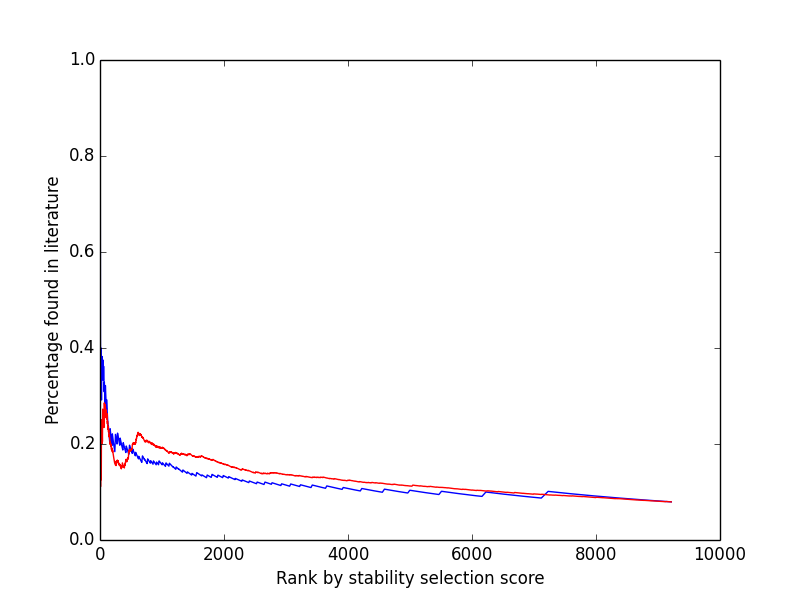
\includegraphics[width=11cm]{predagreement.png}
\caption{Agreement between the list of trigrams, ranked by stability selection score (blue) or by relative frequency(red), and the percentage found in related literature.}
\label{fig:predagreement}
\end{figure}


\begin{figure}[h!]
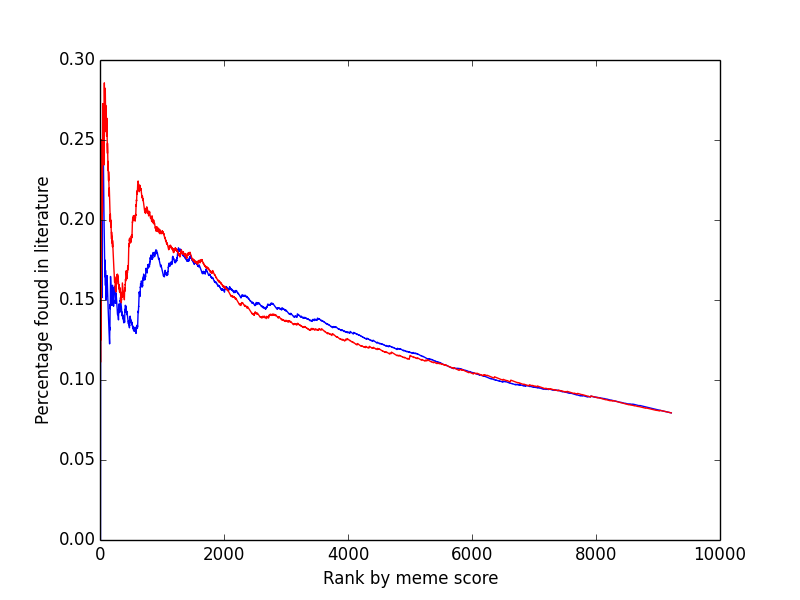
\includegraphics[width=11cm]{memeagreement.png}
\caption{Agreement between the list of trigrams, ranked by meme score (blue) or by relative frequency(red), and the percentage found in related literature}
\label{fig:memeagreement}
\end{figure}

\begin{figure}[h!]
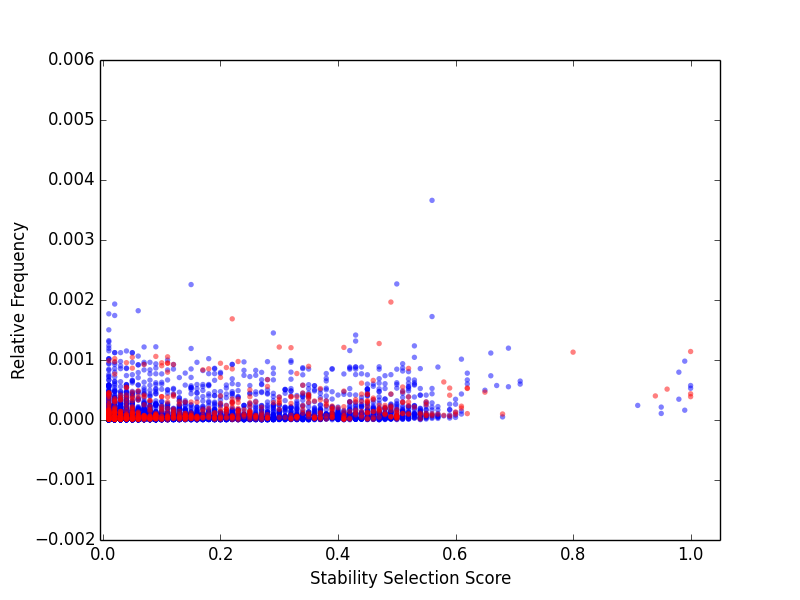
\includegraphics[width=11cm]{predscatter.png}
\caption{Scatterplot of stability selection scores for trigrams, scattered against their frequency in the citation network. Blue dots are not found in related literature, red dots are.}
\label{fig:predscatter}
\end{figure}

\begin{figure}[h!]
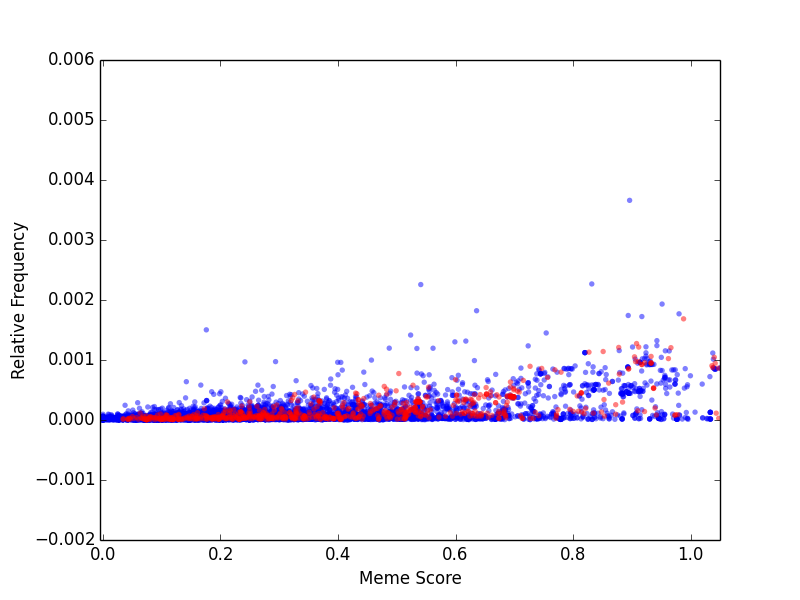
\includegraphics[width=11cm]{memescatter.png}
\caption{Scatterplot of meme scores for trigrams, scattered against their frequency in the citation network. Blue dots are not found in related literature, red dots are.}
\label{fig:memescatter}
\end{figure}




\begin{figure}[h!]
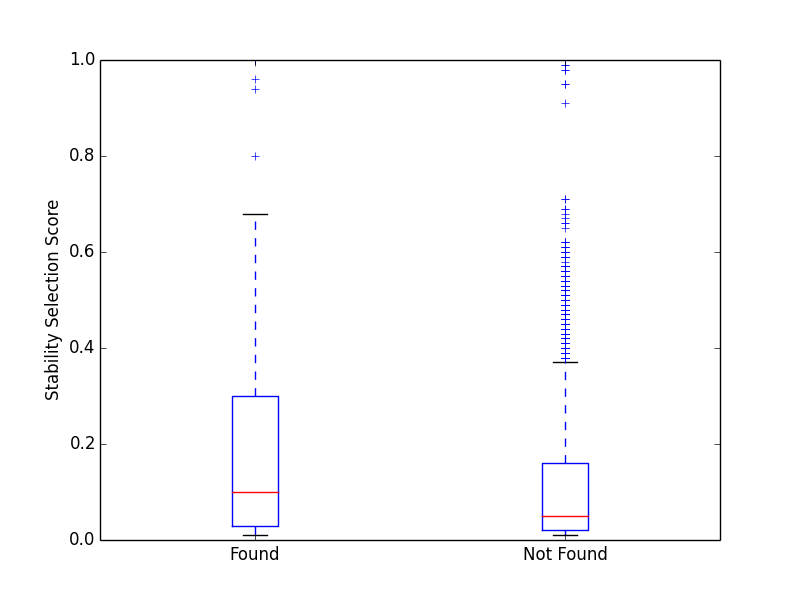
\includegraphics[width=11cm]{predboxplots.png}
\caption{Box plots of relative stability selection scores for Article 10 trigrams, found and not found in related literature}
\label{fig:predbox}
\end{figure}

\begin{figure}[h!]
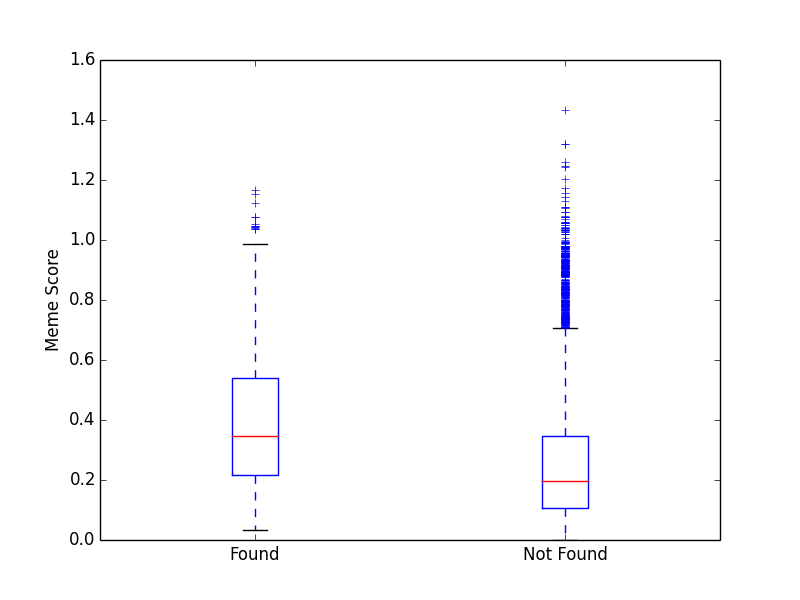
\includegraphics[width=11cm]{memeboxplots.png}
\caption{Box plots of relative meme scores for Article 10 trigrams, found and not found in related literature}
\label{fig:memebox}
\end{figure}

 The scatter plots in figures \ref{fig:predscatter} and \ref{fig:memescatter} show the meme or stability selection score of all trigrams from the article subgraphs used in this section of the experiment (Articles 2, 5, 8, and 10) against their relative frequency in the network and coded red if the trigram is found in the related literature, blue if not. The same relation between meme score and frequency holds as in the previous plots, on account of the formula for calculating the meme score. The blue scattering is plotted first, which may be obscured by the trigrams that are found (red). A cursory look at the two plots suggests a higher amount of trigrams ranked high by meme score, figure \ref{fig:memescatter} that are not found in the literature, and that are relatively frequent in the citation network. \\
 
The boxplots in figures \ref{fig:predbox} and \ref{fig:memebox} compare trigram scoring statistics for grams found in the literature and those not found, for either scoring method. The median of trigrams retrieved through stability selection, in figure \ref{fig:predbox}, that are found in the literature is 0.1, compared to 0.05 for those not found. The median of the data greater than the media of all data (the upper quartile, indicated by the top of the box) is 0.3 and 0.16 for trigrams found and not found, respectively. The lower quartiles are found at 0.03 and 0.02.\\

For trgrams scored by the meme score formula in figure \ref{fig:memebox}, the median for those found is 0.35  compared to 0.2 for those not found. The upper quartile is at 0.54 compared to 0.34 for those not found. The lower quartiles are at 0.21 and 0.1.\\

Figures \ref{predbar} and \ref{memebar} show the percentage of trigrams matched in the literature for the entire ranked list split into 34 bins. The lower the score in \ref{memebar}, the smaller the ratio of memes found in the textbooks. Meanwhile, this seems to not apply to stability selection scores, considering the high percentages in certain low score bins. Given that stability selection scores represent a proportion of times a variable is selected, the values are not continuous. Many low-scoring trigrams will thus end up represented by one specific low score, such as 0.01. 

\begin{figure}[!ht]
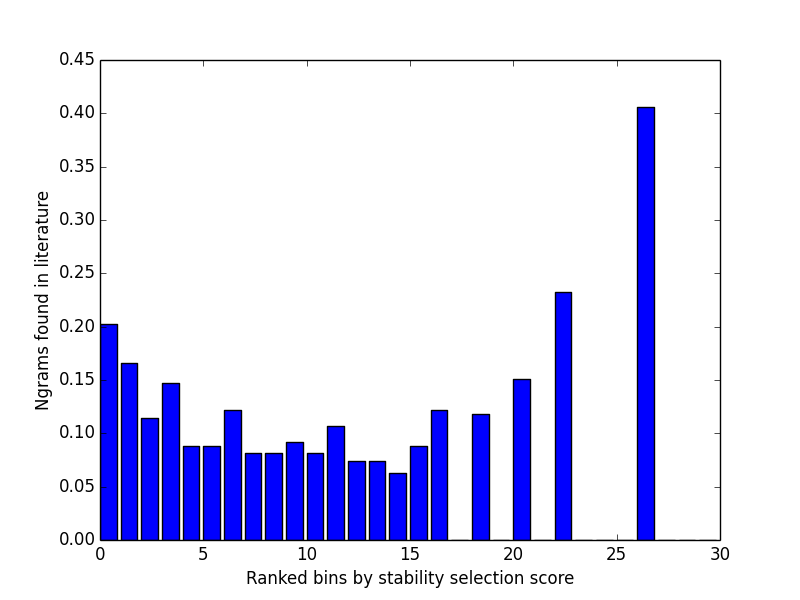
\includegraphics[width=11cm]{predbar.png}
\caption{Ranked stability selection scores binned into 34 sections, each showing the percentage of matched trigrams in that bin.}
\label{predbar}
\end{figure}

\begin{figure}[!ht]
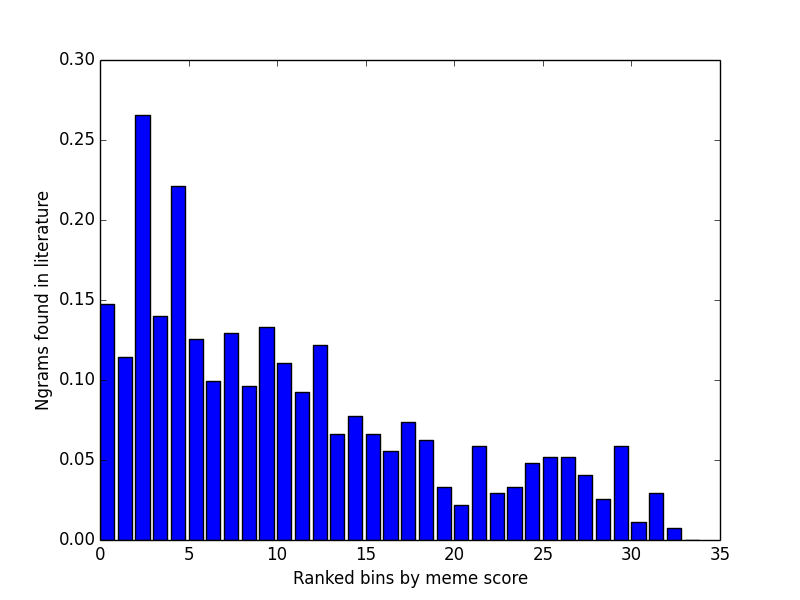
\includegraphics[width=11cm]{memebar.png}
\caption{Ranked meme scores binned into 34 sections, each showing the percentage of matched trigrams in that bin.}
\label{memebar}
\end{figure}



\subsection{Evaluation: Results}

Table \ref{randme} shows the average rank and average score of the random selection of 500 trigrams evaluated by myself, by either method. Scores are consistently higher for trigrams that I had evaluated as related to issues outlined in the literature on Article 10, for both methods of scoring. The average rankings are also consistently better for trigrams I identified over those I did not. \\

Table \ref{agrthem} shows identification and agreement statistics for the annotation task given to two experts in international law. Annotator B was shown to be less conservative in their appraisal of the trigrams relevance to the case law overall. The top 50 stability selection trigrams were identified with at a higher percentage and at a higher rate of agreement for those identified as relevant. Their assessment of the trigrams drawn randomly from outside the top 50 memes or stability selection predictors is more favourable than their evaluation of the top 50 trigrams ranked by meme score. \\

Table \ref{randthem} shows the average scores and rankings of the trigrams drawn randomly from outside the top 50 rankings, whether identified as relevant by one or both annotators or ignored. The average score is higher for trigrams identified by one annotator than the average score of those ignored by both. The average score of trigrams identified by both annotators, retrieved by stability selection, is higher than both single annotator-identified trigrams and those ignored. As for average rankings, a similar relation holds. Ignored trigrams are ranked lower than those identified by both, and individually, except the stability selection ranking assessment of annotator A. The trigrams identified by both are ranked higher on average, except for the average meme score ranking of trigrams identified by annotator A. \\


Tables \ref{predlist} \ref{memelist}, and \ref{randlist} show the trigrams given to the annotators for evaluation, along with their judgment, marked by +, * or *+*+. One noticeable difference between the assessment of meme rankings and stability selection score rankings is how few of the high scoring memes are judged as relevant. Meanwhile the top three trigrams by stability selection score are deemed relevant by both. \\


\begin{table}[h!]
\centering
\begin{tabular}{llll}\hline\hline
 &  & Id'ed & Ignored \\\hline
Avg Random Rank & Meme & 834.8 & 1039.3 \\
 & Stab. Sel. & 917.2 & 1032 \\\hline
Avg Random Score & Meme & 0.33 & 0.27 \\
 & Stab. Sel. & 0.14 & 0.10\\\hline\hline
\end{tabular}
\caption{Average rank and score of identified and ignored random trigrams, my evaluation}
\label{randme}

\end{table}


\begin{table}[h!]
\centering
\begin{adjustbox}{width=\textwidth}
\begin{tabular}{lllll}
\hline\hline
 &  &  & \multicolumn{2}{l}{Identified as relevant} \\\hline
Method & Annotator & Annotator Agreement & Individually & In agreement \\\hline
Meme Score  & A & 78\% & 14\% & 8\% \\
 & B &  & 36\% &  \\\hline
Stab. Select. & A & 76\% & 36\% & 34\% \\
 & B &  & 62\% &  \\\hline
Random & A & 39\% & 23\% & 17\% \\
 & B &  & 44\% & \\\hline\hline

\end{tabular}
\end{adjustbox}
\caption{Identification of top 50 Article 10 trigrams  (by meme score and stability selection scores) and random trigrams, with agreement between annotators}
\label{agrthem}
\end{table}


\begin{table}[h!]
\centering
\begin{tabular}{llllll}
\hline\hline
 & Method & \multicolumn{4}{l}{Annotator} \\\hline
 &  & A & B & Both & Ignored \\\hline
Avg Random Rank \vline & Meme  & 735.3 & 1037.4 & 875.6 & 1062.5 \\
 & Stab. Sel. & 1273.8 & 1011.6 & 918.1 & 1145 \\\hline
Avg Random Score \vline& Meme & 0.38 & 0.25 & 0.32 & 0.24 \\
 & Stab. Sel. & 0.1 & 0.1 & 0.15 & 0.08\\
 \hline\hline
\end{tabular}
\caption{Average rank and score of identified and ignored random trigrams, by evaluators}
\label{randthem}
\end{table}

\begin{table}[h!]
\centering
\begin{adjustbox}{width=\textwidth}
\begin{tabular}{llll}
\hline
 1 limits acceptable criticism *+*+ & 13 enjoy public confidence *           & 25 10 convention ii *                   & 37 expression prescribed law *         \\
 2 subject editorial revision *+*+  & 14 violation article 10 *+*+           & 26 article 11 convention                & 38 governed rule law *                 \\
 3 exercise freedom expression *+*+ & 15 careful scrutiny court *            & 27 certain margin appreciation *        & 39 instituted criminal proceedings +   \\
 4 26 april 1979                    & 16 constitutes essential foundations * & 28 complained light case                & 40 light case including                \\
 5 date procedure case              & 17 person private life *+*+            & 29 field designed cover                 & 41 prior restraints publication *+*+   \\
 6 national authorities justify     & 18 public right receive *              & 30 legitimate aim pursued *             & 42 rights building strasbourg          \\
 7 facts circumstances case         & 19 substance ideas information *+*+    & 31 jurisdiction rights freedoms *       & 43 rule 77 rules                       \\
 8 judgments susceptible proof      & 20 aims prescribed law                 & 32 offend shock disturb *+*+            & 44 society meaning convention *        \\
 9 applying given independent       & 21 applicant freedom expression *+*+   & 33 protection journalistic sources *+*+ & 45 wider limits acceptable             \\
 10 austria judgment strasbourg *   & 22 freedom expression right *+*+       & 34 respect reputation rights *+*+       & 46 restriction freedom expression *+*+ \\
 11 rights freedoms defined *       & 23 human rights building               & 35 section sitting chamber              & 47 substitute views press *+*+         \\
 12 breach article 10 *+*+          & 24 paragraph article 10 *+*+           & 36 bear reasonable relationship         & 48 turkish government government *     \\
 -                                                       & -                                                            & -                                                                & 49 value judgments susceptible  *+*+ \\
  -                                                       & -                                                            & -                                                                & 50 61 echr 1999 \\
 
\hline
\end{tabular}
\end{adjustbox}
\caption{Article 10. Trigrams, top 50 by stability selection score. *+*+ for trigrams identified by evaluators as relevant to the case law. + or * when only relevant to only one evaluator.}
\label{predlist}
\end{table}


\begin{table}[h!]
\centering
\begin{adjustbox}{width=\textwidth}
\begin{tabular}{llll}
\hline
 1 procedure case originated         & 13 editorial revision case *+*+    & 25 power consequently law       & 37 restrictions penalties prescribed    \\
 2 government government represented & 14 article 41 convention           & 26 contrary rule law            & 38 subject formalities conditions       \\
 3 consequently law indicate         & 15 english notified writing        & 27 expressed terms unfettered   & 39 penalties prescribed law *           \\
 4 section sitting chamber           & 16 ill founded meaning +           & 28 terms unfettered power *     & 40 carries duties responsibilities *    \\
 5 sitting chamber composed          & 17 having deliberated private +    & 29 legal discretion granted     & 41 duties responsibilities subject *    \\
 6 measure legal protection *        & 18 delivers following judgment     & 30 defined convention requires  & 42 responsibilities subject formalities \\
 7 section registrar having          & 19 meaning article 35              & 31 convention protection human  & 43 include freedom hold *               \\
 8 rule 77 rules                     & 20 alleged violation article       & 32 protection human rights *    & 44 right shall include                  \\
 9 pursuant rule 77                  & 21 freedom expression right *+*+   & 33 national authorities justify & 45 ii relevant domestic                 \\
 10 77 rules court                   & 22 certain margin appreciation *   & 34 exercise freedoms carries *  & 46 expression right shall *             \\
 11 facts circumstances case         & 23 unfettered power consequently * & 35 shall include freedom *      & 47 ideas interference public *+*+       \\
 12 date procedure case              & 24 discretion granted executive    & 36 freedoms carries duties *    & 48 government represented agent +       \\
  -                                                       & -                                                            & -                                                                & 49 freedom hold opinions  *+*+ \\
  -                                                       & -                                                            & -                                                                & 50 provide accurate reliable  *  \\
\hline
\end{tabular}
\end{adjustbox}
\caption{Article 10. Trigrams, top 50 by meme score. *+*+ for trigrams identified by evaluators as relevant to the case law. + or * when only relevant to only one evaluator.}
\label{memelist}
\end{table}

\begin{table}[h!]
\centering
\begin{adjustbox}{width=\textwidth}
\begin{tabular}{llll}
\hline
 frontiers article shall             & religion foundations democratic *+*+  & convention court immediately            & domestic proceedings government   \\
 hungary european court *            & imposed abolish delay                 & proof requirement prove +               & better position international     \\
 10 based acceptable                 & accordance decision apply             & mr butkevych mrs                        & conflict obligations arising *    \\
 article convention iii              & judgment factual basis +              & embracing legislation decisions         & reputation rights preventing *+*+ \\
 uniform european conception *       & freedom thought conscience *+*+       & broadmindedness democratic society *+*+ & required domestic legislation     \\
 violation committed persons         & communist party turkey *              & consulted agent government              & general state concerned *         \\
 high rate inflation *               & hungarian forints rate                & convention secure jurisdiction          & conscience religion right *+*+    \\
 gc 26682 95                         & domestic courts failed *              & applicant principle sufficient *        & content instrument question *     \\
 expression important everybody *+*+ & subject paragraph applicable          & 11 unless prescribed                    & particular circumstances case     \\
 remainder application admissible    & 10 13 convention                      & security court lack                     & istanbul state security *         \\
 servants offensive abusive *+*+     & procedural guarantees afforded *      & guilt innocence criminal +              & interests public safety *+*+      \\
 cm rec 2007                         & compatible requirements article *     & violated right freedom *                & margin appreciation doing *       \\
 given law facts                     & hearing took place                    & overriding requirement public *+*+      & law european court                \\
 regardless frontiers exercise       & administration justice intermediaries & religion beliefs shall *                & mass media shall *+*+             \\
 02 april 2006                       & importance freedom expression *+*+    & relevant provisions constitution        & incurred domestic proceedings     \\
 concerned gc 26682                  & consonant requirement article         & required establishing offence +         & bulgaria lodged court *           \\
 convention reasons court            & submitted parties summarised          & redress breach convention *             & foighel mr loizou                 \\
 context public debate *+*+          & set forth article                     & paragraph article 11                    & matters public concern *+*+       \\
 executive expressed terms           & level justifiable principle *         & faith order provide *                   & just pay concerned                \\
 received regarded inoffensive +     & prescribed law 35                     & ballot conditions ensure +              & european supervision regards *    \\
 obligation article convention       & need appropriate advice               & interferences public authorities *+*+   & reasons court unanimously         \\
 level rights needs                  & interference corresponded pressing *  & assessment necessity measure *          & 10 protects substance *+*+        \\
 chargeable applicant respect        & right freedom thought *+*+            & domestic law practice                   & convention russian national *     \\
 pressing social need *              & purposes article 10 *+*+              & partial reparation consequences *       & russian government government *   \\
\hline
\end{tabular}
\end{adjustbox}
\caption{Article 10. Random Selection of Trigrams. *+*+ for trigrams identified by evaluators as relevant to the case law. + or * when only relevant to only one evaluator.}
\label{randlist}
\end{table}




\section{Discussion}
My link prediction experiments confirm that the approach taken for ranking ngrams by stability score is reliable. The overall F-1 scores range from 82\% to 90\% for logistic regression models trained only on the intersection of vocabularies. Adding additional features from the network's metadata or network structure provides little to no improvement. Both scoring methods produce rankings that in some ways reflect how the case law has been described in related literature. Trigrams that are matched with trigrams from guidebooks about the law are ranked higher than those that are not matched. Evaluations by myself and experts on Article 10 trigrams reveal a similar pattern. The trigrams we ignored were, on average, trigrams to which both methods assigned a lower score. \\

The rankings returned on the Article 10 subgraph were, however, not judged to provide a very precise reflection of the case law on Article 10 by the expert annotators. Both annotators ignored a large section of the top 50 trigrams for either method, but especially those retrieved by meme score, which was favoured at a lower rate than the random sample of trigrams from outside the top 50. Agreement on trigrams deemed relevant was also very low (8\%, 34\%, and 17\%).\\ 

At a minimum, both scoring methods capture something about the citation dynamics. Tracking how ngrams propagate through a network, combined with their frequency, does give an indication of the language used in important cases and points to ideas that define the case law. Similarly, predicting whether or not a judgment ought to cite another based on the language they share can illustrate the jurisprudence, by identifying which words are most predictive of citation. \\

Given the results of my evaluation experiments, one may suspect that a more accurate mapping of the language that is important to the case law could be produced through different methods. Are predictive variables for a link prediction task and high propagating ngrams the best measures of how case law has developed? The following sections will describe my efforts to answer this question given two scenarios. One could assume that the two approaches can produce ranked lists of ngrams that capture the court's history accurately, but that my exact methodology failed to do so. An analysis of potential weaknesses in my approach will follow. One could alternately imagine that my method, relying on the texts associated to a citation network and statistics derived from their connections, is empirically grounded and operates with a more comprehensive view of the jurisprudence than either experts or case law literature. This would assume that the guidebook authors could not be as systematic in their assessment of the case as my method. This scenario will also be examined below. \\


Some additional preprocessing steps could have been taken to prevent the model from considering certain ngrams entirely. A look at the top 50 trigrams for Article 10 shows a high proportion of trigrams that were ignored by the annotators, seemingly on account of the prevalence these trigrams would have across all judgments texts. Ngrams such as ``date procedure case'', ``facts circumstances case'', ``human rights building'', ``section sitting chamber'' are listed within the top 25. These represent expressions found in potentially every judgment text, detailing the date of the procedure or as a heading for a section of the text. The model seems to have picked up a pattern where no significance ought to be attributed. The legal boilerplate of the judgment headings might display small variations. A cursory examination of the data shows many if not all judgments begin with a listing of the judges, expressed as ``sitting as a chamber''. This trigram also appear as the fifth highest ranked meme. A thorough comparison of a selection of judgement texts also reveals an inconsistent use of the heading ``The Circumstances of the Case'', at times omitted. A similar preponderance of expressions tied to the administration of the court, independent of the case, is found in the top memes. Notably, Article 10 trigrams lists very similar memes at the 8th, 9th and 10th position: ``rule 77 rules'', ``pursuant rule 77'', ``77 rules court''. These refer to a rule by which the judgment must be signed by the President of the Chamber and the Registrar. Consequently, most documents, if not all, are signed, ``pursuant to this rule''. The formula used for calculating an ngram's meme score ought to reveal expressions that are important and interesting to the subgraph. Potential improvements on the formula could come from optimizing the amount of controlled noise added. The authors in \cite{kuhn2014inheritance} perform a thorough comparison of different noise levels, and similar experiments could benefit my approach.\\


It is possible that small changes in the use of these expressions over the history of the court create an association to citation, which both methods pick up as a pattern. A better approach might reformulate the meme score calculation to include a temporal dimension, and may train different models for different time periods. This could prevent results provided by ``boilerplate drift'', while also controlling for a potential concept drift. Under a static view of the citation network, variables are given a weight with no consideration for fluctuation across time in the citation network. It is possible that once case law is settled, citation patterns change over time. Previous research has shown that precedent at the US Supreme Court eventually depreciates \cite{black2013citation}. Do certain rights and freedoms enjoy a protection that has gone uncontested in recent decades, but whose early defence spawned considerable jurisprudence? A model trained on the citation network in a dynamic manner may provide more meaningful and interpretable results. An approach similar to the time-series regularization used in \cite{yogatama2011predicting} could be an approach of interest for future work on this data. 

Another improvement could handle the insufficient precision in the representation of citation in the network. The modelling and meme score calculation predict and consider links between judgments without differentiating between various motivations for citation. As noted in \cite{whalen2016legal}: \begin{quote}(\ldots)we know that judges include these in their opinions for many different reasons. They are used to provide authority for a rule interpretation, distinguish a case from a similar precedent, note the existence of binding precedent, or for many other reasons.\end{quote}
In attempting to describe the case law by automatically extracting key words that are either predictive of or highly aligned with citation, a binary understanding of citation may limit accuracy of this mapping. One solution may involve a network with weighted edges, to account for different degrees of commitment to precedent by the citing judge. Similarly, a citation network, in which nodes correspond to the contexts of citation rather than the entire judgment text would provide more detailed citation patterns. Modeling a paragraph-to-paragraph citation network (with weighted edges) would prevent the model from picking up irrelevant ngrams in the shared vocabulary and hint at the motivation behind the citation.  \\

Returning to approaches that are feasible given the data at hand, a better ranking by meme score and stability selection score may be achieved by modelling and calculating important unigrams, bigrams and trigrams together. Optimizing stability selection parameters should be considered as well.  A better match between ngrams returned and ngrams found in the literature may result from a higher number of randomized models, a different sampling fraction and a different scaling value. \\

The propagation of different ngrams through the citation network is analogous to the replication of genes in living organisms, as the memetic framework implies. One can play with different extensions of this analogy, viewing citation as the passing on of genes and sentences or documents as DNA. It is undetermined whether differences in exact wording of the issues linking one judgment to another represent ``meme mutations'' or a further analogy to the interplay between genotypes and phenotypes (the gene vs how it is expressed). Previous work has made the case for different syntactic and morphological expressions of a meme to be considered as involving a similar interaction \cite{fried1999evolution}. The semantic content of the issue is what is meant to be captured by an approach informed by memetics. Different steps taken to arrive at a more abstract representation of the meme may track its propagation in the network more exactly. My experiments have gone so far as to remove stop words between units of trigrams and bigrams. Different morphological expressions, through derivation or inflection, could be controlled for by an additional stemming step in the preprocessing stage. \\

An alternate manner of assessing the results of my different validation steps, in which many high scoring ngrams were either ignored by myself or experts and not matched to ngrams in the literature, is to assume that my rankings provide a better mapping of the case law than textbooks or the experts participating in the annotation task. The raison d'�tre of a computational approach relying on statistics from the citation network and associated texts is to arrive at an understanding of the data that is empirically grounded, free from subjective human biases that may impact the choices made in writing a guidebook on the case law. It may be worth examining my results under this hypothesis. I have no way of testing how comprehensive my participants' knowledge of the law may be, so their evaluation will be left aside. I have produced in table \ref{memepred10} a list of trigrams extracted from the Article 10 subgraph that were not matched in the literature. The top of the meme score rankings and stability selection score rankings were combined, and the value at every trigrams corresponds to a combination of the trigram's meme rank and stability selection rank. The list is low on substantive issues. What was not matched in the literature appears to mostly be noise from either method, representing expressions from the administration of the court. Trigrams that seem to refer to a legal issue or case are, from my interpretation of the case law, adequately addressed in textbooks, with potentially different wording.\\

One could potentially conclude that the textbooks on Article 10 adequately covered the case law and that any discrepancy between the results of my modelling and propagation scoring with the literature is a result of my approach. A quick examination of combined rankings for another area of the law may however lend support to the superiority of my approach. The focus given to Article 10 and the freedom of expression in my evaluation experiments is a result of discussions with experts in international law. Article 10 case law is supposedly recognized as having been thoroughly described by the textbooks. This may help explain the lack of substantive legal issues in the unmatched trigrams. Article 8, which protects the right to respect for private and family life, makes up a sizeable proportion of the citation network. I have listed the trigrams that were not matched with trigram in the literature on Article 8, and ranked them by combined meme and stability selection score. Although I have not familiarized myself with this area of the law, the results of this ranking offer a slightly different picture. Within the top 25 unmatched trigrams, there are considerably more expressions referring to substantive legal issues, over procedural or boilerplate trigrams. Among others:``measure basis domestic'', ``security remand centre'', ``objective reasonable justification'', ``constitute fundamental elements'', ``duration treatment physical'', ``ukraine lodged court'', ``measure judged swiftness''. \\

A more thorough comparison of the omissions of legal issues from textbooks would require a more informed hypothesis as to what areas of the law may be understudied, and equivalent evaluation experiments for either results. Nevertheless, my approach, which involves extracting and ranking the legal language associated to patterns in a citation network may provide a more descriptive and empirically grounded method for future comparisons of the case law and texts meant to outline its content.\\


\begin{table}[h!]
\centering
\label{my-label}
\begin{adjustbox}{width=\textwidth}
\begin{tabular}{llll}
\hline
 15 date procedure case            & 393 light case including            & 640 construed strictly need          & 795 investigation capable leading         \\
 37 section sitting chamber        & 406 26 april 1979                   & 641 assembly guaranteed article      & 796 republic austria lodged               \\
 49 rule 77 rules                  & 424 reasons court unanimously       & 655 wanted proceedings continue      & 808 law implies qualitative               \\
 72 pursuant rule 77               & 453 turkish government government   & 664 serbia judgment strasbourg       & 809 read follows article                  \\
 87 10 convention ii               & 460 shall placed exercise           & 664 discretion granted executive     & 815 echr 1999 iv                          \\
 97 procedure case originated      & 473 minimum level severity          & 678 light case decisions             & 822 leading identification punishment     \\
 111 subject editorial revision    & 490 freedoms convention russian     & 679 opinions acquire disseminate     & 831 circumstances absolving requirement   \\
 111 sitting chamber composed      & 491 turkey european court           & 679 power consequently law           & 835 serbia european court                 \\
 130 77 rules court                & 496 afford just satisfaction        & 685 rule admissibility merits        & 843 terms unfettered power                \\
 154 article 11 convention         & 502 61 echr 1999                    & 695 accordance article 44            & 848 identification punishment responsible \\
 167 article 35 convention         & 519 convention subject editorial    & 696 linked prevention terrorism      & 855 russian federation european           \\
 172 rights building strasbourg    & 521 section registrar having        & 697 3002 03 23676                    & 856 committed offence reasonably          \\
 199 judgment adopted date         & 528 look interference complained    & 699 field designed cover             & 861 adopted mentioned date                \\
 215 court shall necessary         & 546 breach article 11               & 702 convention notes inadmissible    & 861 44 convention subject                 \\
 230 allow unduly influenced       & 553 decided rule admissibility      & 710 application republic turkey      & 862 primarily matter individual           \\
 260 complained light case         & 562 unfettered power consequently   & 727 austrian government government   & 868 duty loyalty reserve                  \\
 261 court allow unduly            & 563 task exercising supervisory     & 740 reasonable doubt applicant       & 870 interference infringe convention      \\
 267 shall necessary afford        & 580 information expressed form      & 742 gazette republic serbia          & 870 applicant establish remedy            \\
 272 allows partial reparation     & 589 genuine effective exercise      & 744 republic turkey lodged           & 871 number status addressed               \\
 285 secure jurisdiction rights    & 604 expressed form conveyed         & 755 expressed terms unfettered       & 876 regarded objectively justified        \\
 286 editorial revision case       & 605 03 23676 03                     & 761 case law purpose                 & 877 authority reasonable suspicion        \\
 287 adopted date procedure        & 612 dismisses unanimously remainder & 777 person concerned foreseeable     & 880 designed cover number                 \\
 322 mentioned date procedure      & 616 government represented mr       & 790 concerned foreseeable effects    & 882 society meaning convention            \\
 327 interference complained light & 630 152 civil code                  & 790 30 june 2004                     & 882 matter individual conscience          \\
 355 rigorous european supervision & 632 article 152 civil               & 792 implies qualitative requirements & 885 law purpose domestic                  \\
\hline
\end{tabular}\end{adjustbox}
\caption{Article 10. Trigrams unmatched in literature, with combined meme and stability selection rank.}
\label{memepred10}
\end{table}



\begin{table}[h!]
\centering
\label{my-label}
\begin{adjustbox}{width=\textwidth}
\begin{tabular}{llll}
\hline
 35 measure basis domestic              & 427 kodeks karny wykonawczy       & 586 high contracting party              & 735 bank default period              \\
 39 procedure case originated           & 442 adequacy measure judged       & 591 plus tax chargeable                 & 740 convention violated shall        \\
 45 editorial revision case             & 444 subjected torture inhuman     & 600 facet individual existence          & 751 utmost importance effective      \\
 84 date procedure case                 & 464 assist maintaining contact    & 613 shall secured discrimination        & 751 capable humiliating debasing     \\
 114 article 35 convention              & 479 civil aspects international   & 616 anguish inferiority capable         & 755 polish national mr               \\
 115 subject editorial revision         & 482 code criminal procedure       & 621 society order achieve               & 759 inferiority capable humiliating  \\
 164 section sitting chamber            & 484 life meaning article          & 626 judged swiftness implementation     & 762 forth convention violated        \\
 185 mentioned date procedure           & 486 reasons court unanimously     & 629 secured discrimination ground       & 763 imprisonment ordinary regime     \\
 233 adopted date procedure             & 491 sitting chamber composed      & 637 existence identity stake            & 764 satisfaction injured party       \\
 240 security remand centre             & 498 present day conditions        & 639 article 14 taken                    & 772 community contexts state         \\
 244 allows partial reparation          & 501 case duration treatment       & 650 entitled trial reasonable           & 774 process leading measures         \\
 253 objective reasonable justification & 506 code execution criminal       & 663 difference treatment discriminatory & 776 45 convention rule               \\
 255 constitutes fundamental element    & 514 shall subjected torture       & 669 reasonable time release             & 778 cases accordance procedure       \\
 258 states council europe              & 520 torture inhuman degrading     & 670 judgment adopted date               & 786 rule 74 rules                    \\
 288 english notified writing           & 525 adopted mentioned date        & 672 time release pending                & 787 period plus percentage           \\
 347 measure judged swiftness           & 527 right protection reputation   & 672 having deliberated private          & 789 just satisfaction injured        \\
 357 duration treatment physical        & 530 authority disposal remains    & 696 24 march 1988                       & 791 application article 37           \\
 360 application article 14             & 551 convention subject editorial  & 698 shall entitled trial                & 799 convention shall secured         \\
 366 fundamental element family         & 555 reside particular country     & 700 section registrar having            & 809 merits application time          \\
 383 rights building strasbourg         & 559 knew ought known              & 701 violated shall effective            & 812 explicit procedural requirements \\
 398 company constitutes fundamental    & 560 execution criminal sentences  & 708 notes inadmissible grounds          & 819 importance effective operation   \\
 400 judgment adopted mentioned         & 568 number family visits          & 708 default period plus                 & 822 violation article 13             \\
 409 ukraine lodged court               & 573 mutual enjoyment parent       & 716 afford just satisfaction            & 835 74 rules court                   \\
 412 contains explicit procedural       & 575 appeared court government     & 719 say justified pressing              & 841 ill treatment attain             \\
 422 44 convention subject              & 579 serving sentence imprisonment & 729 forth convention shall              & 845 release pending trial            \\
\hline
\end{tabular}
\end{adjustbox}
\caption{Article 8. Trigrams unmatched in literature, with combined meme and stability selection rank.}
\label{memepred8}
\end{table}




\section{Conclusion and Future Work}
This dissertation presented experiments in which I attempted to automatically extract key phrases from the citation network of the European Court of Human Rights. I employed two different approaches to systematically characterize the citation network of the ECHR by providing scored ngrams, ranked by their propagation in the citation network and by their proportion of times selected through stability selection of randomized logistic regression models of the network. Whereas previous work performing legal network analysis has examined citation patterns, my approach incorporates language use into the study of precedent. The two scoring systems can be used by legal scholars hoping to support their doctrinal analyses with advanced statistical methods of word usage in the citation network or the ECHR. I have also conducted a series of link prediction experiments, showing that textual content is equally, if not more, predictive of citation as metadata and network structure features. \\

A series of validation experiments reveal that my two methods are reliable to capture citation dynamic within the network. Both experts and I tended to identify trigrams related to Article 10 as relevant when their meme score and stability selection score was higher. The recall and agreement of the annotators was not especially high, however. A validation stage of comparing ngrams with the literature on their respective case law reveals similar patterns. Ngrams matched in the literature had higher scores and ranks than those that did not match. Unmatched ngrams from both the meme score rankings and stability score rankings can be listed on account of their combined ranks and compared to rerankings of different areas of human rights law, in order to gauge which area is understudied. \\

Future work should consider modelling and measuring memes in the citation network dynamically; the network and its associated texts should be split into different periods to capture trends in key phrase use and a more exact mapping of the case law. An approach involving weighted edges could also provide for more detailed results, considering the different motivations behind references to precedent. Finally, more thorough preprocessing can be conducted to remove boilerplate and to employ more abstract representations of the key phrases.\\

\section{Article 10: Freedom of Expression }



\begin{quote}	1. Everyone has the right to freedom of expression. This right shall include freedom to hold opinions and to receive and impart information and ideas without interference by public authority and regardless of frontiers. This article shall not prevent States from requiring the licensing of broadcasting, television or cinema enterprises.\\

	2. The exercise of these freedoms, since it carries with it duties and responsibilities, may be subject to such formalities, conditions, restrictions or penalties as are prescribed by law and are necessary in a democratic society, in the interests of national security, territorial integrity or public safety, for the prevention of disorder or crime, for the protection of health or morals, for the protection of the reputation or rights of others, for preventing the disclosure of information received in confidence, or for maintaining the authority and impartiality of the judiciary \cite{harris2014harris}.\\
\end{quote}
The second volume of the human rights handbooks, 'Freedom of Expression: A guide to the implementation of Article 10 of the European Convention on Human Rights', goes over the important case-law surrounding this article and its associated doctrines, principles and concepts \cite{macovei2004guide}. The intended audience of the guidebook is judges, both at national levels and at the ECHR, as the case law is summarized for the purpose of guaranteeing a level of consistency across member states and within the court itself.  The guidebook begins with some general considerations on freedom of expression and goes on to evaluate the manner in which judges have interpreted both paragraphs of article 10. The following summarizes the guidebook, laying out the potential keywords and phrases that seem to reflect core concepts in Article 10 jurisprudence.\\

Freedom of expression aligns with freedom of assembly, while being potentially at odds with rights such as the freedom of conscience and religion and the right to respect for private life. Jurisprudence on freedom of expression has weighed conflicting rights with an emphasis on how freedom of expression is important to democratic society, progress and individual self-fulfillment. Also important is the pre-eminent role of the press. Expression is protected regardless of its content, unless what is expressed negatively affects other rights and freedoms, or invites racism, hatred or Nazism. The court is then faced with the paradox of tolerance, i.e., can intolerance become the result of allowing absolute tolerance in expression.\\

When a state has interfered with freedom of expression, considerations that may contribute to a justification of this interference include the type of expression, the means of dissemination, the audience, and the truth of the expression.\\

The freedom to hold opinions, established in paragraph 1 of Article 10, also leads to a freedom of not being forced to express this opinion. The paragraph 1 freedom to impart information and ideas involves concepts such as the public interest, artistic freedom and how creative work shapes public opinion. The state cannot interfere between the media and its audience \cite{macovei2004guide}.\\

The court also considers how the truth of value judgments differs from the existence of facts and how this applies to a crime of insult and defamation. It looks at the proportionality of an interference, and whether there is enough truth to the expression. The right to receive information involves the right to be adequately informed. Freedom of the press and its role as a political watchdog ties in with ideas of political debate and political issues, and these ideas are weighed when the press may affect the reputation of others through rumours and allegations. Objectivity and the protection of sources are other factors. Paragraph 1 covers the right of the State to require broadcasting licenses. This prevents monopolies and ensures a a diversity of information, responding to the needs of the public\\

The jurisprudence is particularly concerned with protecting expression that might offend or use strong language, regardless of the form of the expression ' whether in writing, spoken or in picture. The court has drawn the line at expression that incites violence.\\

Freedom of expression is therefore not an absolute right, and the second paragraph of Article 10 covers potential justifications for restrictions on this freedom. Civil servant and state employees are not free in the same way as private citizens due to responsibilities and status stemming form their profession. Judges are expected to preserve their impartiality by limiting themselves in their public expression. However, confidentiality can only be expected of civil servants for particular categories of information. Information can only be restricted if national security is actually threatened. Journalists are other professionals who have responsibilities such as ensuring that the information they share is accurate\\\

Paragraph 2 is concerned with the different ways in which a state may restrict freedom of expression, whether conviction, forcing to reveal sources, fines or censorship, which is a special concern as it restrains expression before it happens. Certain punishments have led to an examination of the government's dominant position and the proportionality of the interference on freedom of expression. The Court has expressed a desire to protect sources, as they may avoid talking to the media if they lose their anonymity. Censorship as well as fines and trial expense may also impede on the work of press unjustly \cite{macovei2004guide}. \\

The second paragraph outlines criteria for interfering with freedom of expression, such as protecting the reputation of others and national security. The court has however emphasized a strict interpretation of these criteria, in that restrictions must be based on these criteria only. Any law restricting freedom of expression has to be published and accessible, and precise enough for individuals to govern themselves accordingly. \\

The image or honor of a country is not covered as a reason for interference, nor are state prestige and authority. The reputation of high officials should not be protected with higher penalties. And threats to national security must be real and not an uncertain possibility. \\

Interference as a means to restrict freedom of expression must have an aim that is proportional to the means of the interference. It must respond to a ``pressing social need''. The second paragraph lists potential aims, and jurisprudence has developed to define them.\\

When the aim is the protection of national security, the court has found that confidential information may be restricted, but has found that once the information is released and has been received by the public, further limitations on sharing its content is unjustified. The court also considered whether the interest of the public in having the information is more important than national security. On issues of conflict in Turkey, has differentiated writing that encourages violent means from communication that criticizes the state's actions \cite{macovei2004guide}.\\

When a government acts in a way to prevent disorder and crime, the court examines similar considerations. Was the expression an incitement to violence or terrorism or an exercise in scrutiny of the government, and was the punishment disproportionate. Can military personnel be punished for engage in a discussion of ideas about the army, or does that threaten the system of defense.\\

 
As for restrictions based on protecting the reputation of others, the court has prioritized the freedom of the press and political debate over the reputation of politicians, who are expected to be criticized.  Pubic discussion depends on media criticism and either censure or punishments after an article is shared may have a chilling effect. Nor can a journalist's value judgments be tested on their truth. A potentially offensive article can be protected by concerns such as the ``free debate of ideas'' and exaggeration can be allowed. Whether or not a journalist intended to defame someone is another consideration as are the purpose and impact of an article. Civil servants, on the other hand, were considered not to carry the same expectation of being closely scrutinized \cite{macovei2004guide}.\\

When the court has weighed freedom of expression over the right to religion, it is expected that religion can be criticized and denied. But expression that offends the religion without any particular purpose is condemned, such as portrayals of religious objects in an unnecessarily negative offensive light.\\

The court has also found that restrictions on racist expressions would not be upheld when the purpose is not propagation, but to expose and analyze these views through journalism, with no say in how balanced or objective the report may be. The court has also protected expressions against judicial authorities, which may have been limited to preserve public trust. The court recognized the impossibility of preventing prior discussion of disputes, outside the judicial system, which it argues cannot operate in a vacuum. Criticism of judges' independence or impartiality should not automatically be restricted either.\\


\bibliographystyle{ieeetr}
\bibliography{biblo}

\end{document}
